% !TEX root = Thesis.tex
\chapter{Experimental Results}\label{chap:Exp}

  Our layout migration framework is implemented in c++ language on Intel 5420 Quad Core 2.5GHz machine under Linux CentOS 5.8 platform. We apply OpenAccess v22.04p54 for extracting industrial design and using Synopsys PyCell Studio for layout generation. Three experimental circuits are practiced as our reference layouts: (1) A folded-cascode operational amplifier (OpAmp) design, (2) a variable-gained amplifier (VGA) under umc90nm, and (3) a low drop-out regulator (LDO). 

  %\begin{table}[ht]
  %    \begin{center}
  %    \scriptsize
  %    \caption{Specification of experimental circuits: OpAmp and VGA}\label{table:Spec}
  %    \begin{tabular}{|l|c|c|}
  %    \hline
  %      Circuit   & OpAmp & VGA \\ 
  %      \hline
  %      technology  & umc90nm & umc90nm     \\
  %      \hline
  %      $V_{dd}$     & 1V    & 1.1V        \\
  %      \hline
  %      Load Capacitance  & 200pF & 1.5pF   \\
  %      \hline
  %      Gain    & $\geq 48.653dB$ & $\geq 18.48dB$      \\
  %      \hline
  %      Gain Bandwidth &  $\geq 100 MHz$ & $\geq 5MHz$      \\
  %      \hline
  %      Phase Margin  & $\geq 45deg$ & $\geq 45deg$     \\
  %      \hline
  %      Area    & 832.66 $\mu m^2$  & 10889.88 $\mu m^2$  \\
  %    \hline
  %    \end{tabular}
  %  \end{center}
  %\end{table}

  \definecolor{mygray}{gray}{.9}
  \begin{table}[ht]
    \scriptsize
    \begin{center}
      \caption{Invalid crossing edges and crossing points of migrated crossing graph comparing to original crossing graph}\label{table:CrEdgeChanged}
      \begin{tabular}{|c|c|c|c|c|m{1.2cm}|}
        \hline
          Tech. & layout & \#Invalid CrEdge & \#Invalid CrPoint\\
        \hline
        \rowcolor{mygray}
        \multicolumn{4}{|c|}{Opamp: \#TriEdge=150, \#CrEdge=83, \#CrPoint=193} \\
        \hline
        \multirow{8}{*}{umc65nm} & Topo1 & 0 & 0 \\
        \cline{2-4}
        & Topo2 & 31 & 23 \\
        \cline{2-4} 
        & Topo3 & 20 & 10 \\
        \cline{2-4}
        & Topo4 & 0 & 0 \\ 
        \cline{2-4}
        & Topo5 & 24 & 37 \\
        \cline{2-4}
        & Topo6 &15 & 24\\
        \cline{2-4}
        & Topo7 & 46& 61 \\
        \cline{2-4}
        & Topo8 & 11 & 15 \\
        \hline
        tsmc90nm & Topo1 & 4 & 11 \\
        \hline
        \rowcolor{mygray}
        \multicolumn{4}{|c|}{VGA: \#TriEdge=353, \#CrEdge=249, \#CrPoint=810} \\
        \hline
        umc65nm & Topo1 &  95 & 298 \\
        \hline
      \end{tabular}
    \end{center}
  \end{table}

  In the following experiments, we intend to show the ability of layout reusability by our migration flow. Therefore, we compare several migrating techniques as below: 

  \begin{itemize}
    \item {\bf \cite{msc-bhattacharya-tcad06}}: Placement migrated into targeting technology and the corresponding routing is accomplished by manual routing.
    \item {\bf \cite{ALP_YPWeng_iccad2011}}: Placement migrated into targeting technology with multiple topologies. The producing placements partially preserved the constraints including symmetry, matching and proximity with respect to the original layout.
    \item {\bf \cite{Chin_DMR_ICCAD2013}}: Routing migrated into targeting technology based on CDT preservation. If the topology of placement changes, the relationship among wires and modules can be partially preserved and reconnected.
    \item {\bf RtMaMi}: Routing manually migrated into targeting technology. 
    \item {\bf RtNoMi}: Routing is not migrated into targeting technology. A simple maze routing is applied to connect the wires. 
    \item {\bf Ours:}  Our approach is a mixed version of \cite{ALP_YPWeng_iccad2011}, \cite{Chin_DMR_ICCAD2013} and {\it Wire Segment Refinement} which is implemented for better performance.
  \end{itemize}

  We first practice the proposed migration framework to layout generation towards different technologies in Section~\ref{sec:ExpMigration}. Later, a comparison among multiple migrated placements with different routing migrating techniques is demonstrated in Section~\ref{sec:ExpMultiProto}. The specifications of the source layouts for OpAmp and VGA in Section~\ref{sec:ExpMigration} and Section~\ref{sec:ExpMultiProto} are the same as Table I in \cite{Chin_DMR_ICCAD2013}. In addition, Table~\ref{table:CrEdgeChanged} notes the number of invalid crossing edge and invalid crossing point for each layout after migration. In brief, the fewer invalid crossing edges and invalid crossing points, the more reusability of the updated crossing graph.


  \begin{figure}[ht]
      \centering
        \begin{subfigure}[t]{0.4\textwidth}
        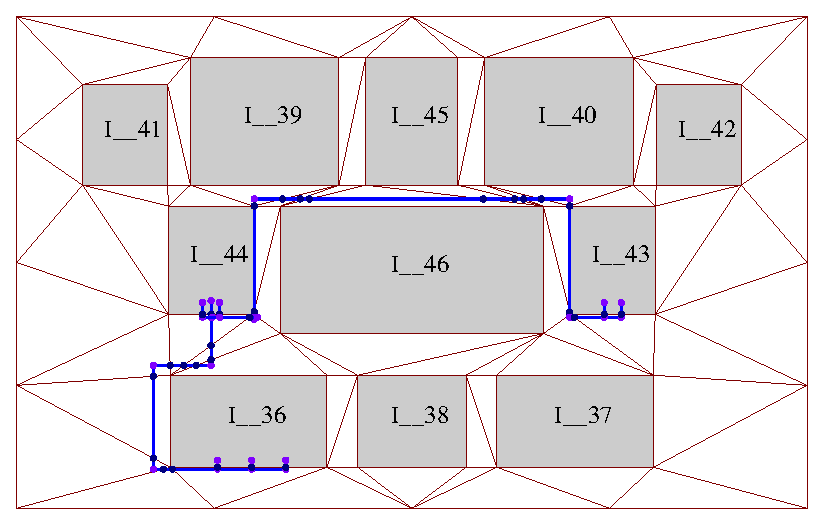
\includegraphics[width=\textwidth]{Fig/OrigOpamp.eps}
        \caption{OpAmp umc90nm}\label{fig:OrigOpamp}
        \end{subfigure}
        \begin{subfigure}[t]{0.4\textwidth}
        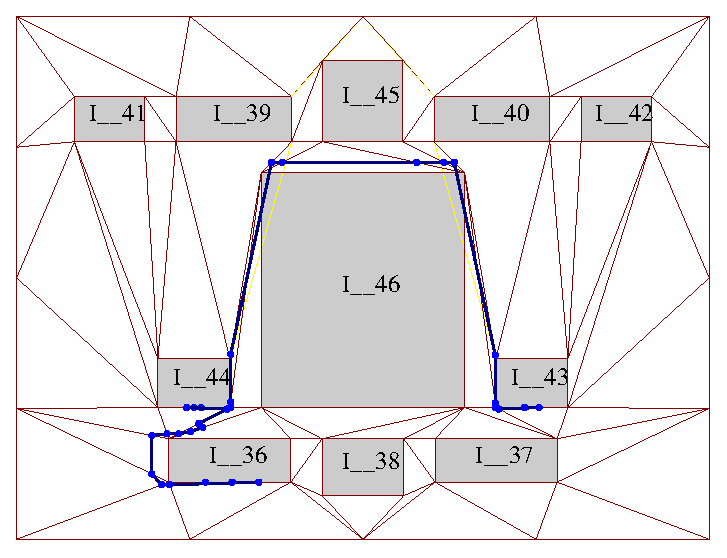
\includegraphics[width=\textwidth]{Fig/OpampProto.eps}
        \caption{OpAmp tsmc90nm}\label{fig:OpampProto}
        \end{subfigure}
        \begin{subfigure}[t]{0.4\textwidth}
        \includegraphics[width=\textwidth]{Fig/OrigVGA.eps}
        \caption{VGA umc90nm}\label{fig:OrigVGA}
        \end{subfigure}
        \begin{subfigure}[t]{0.4\textwidth}
        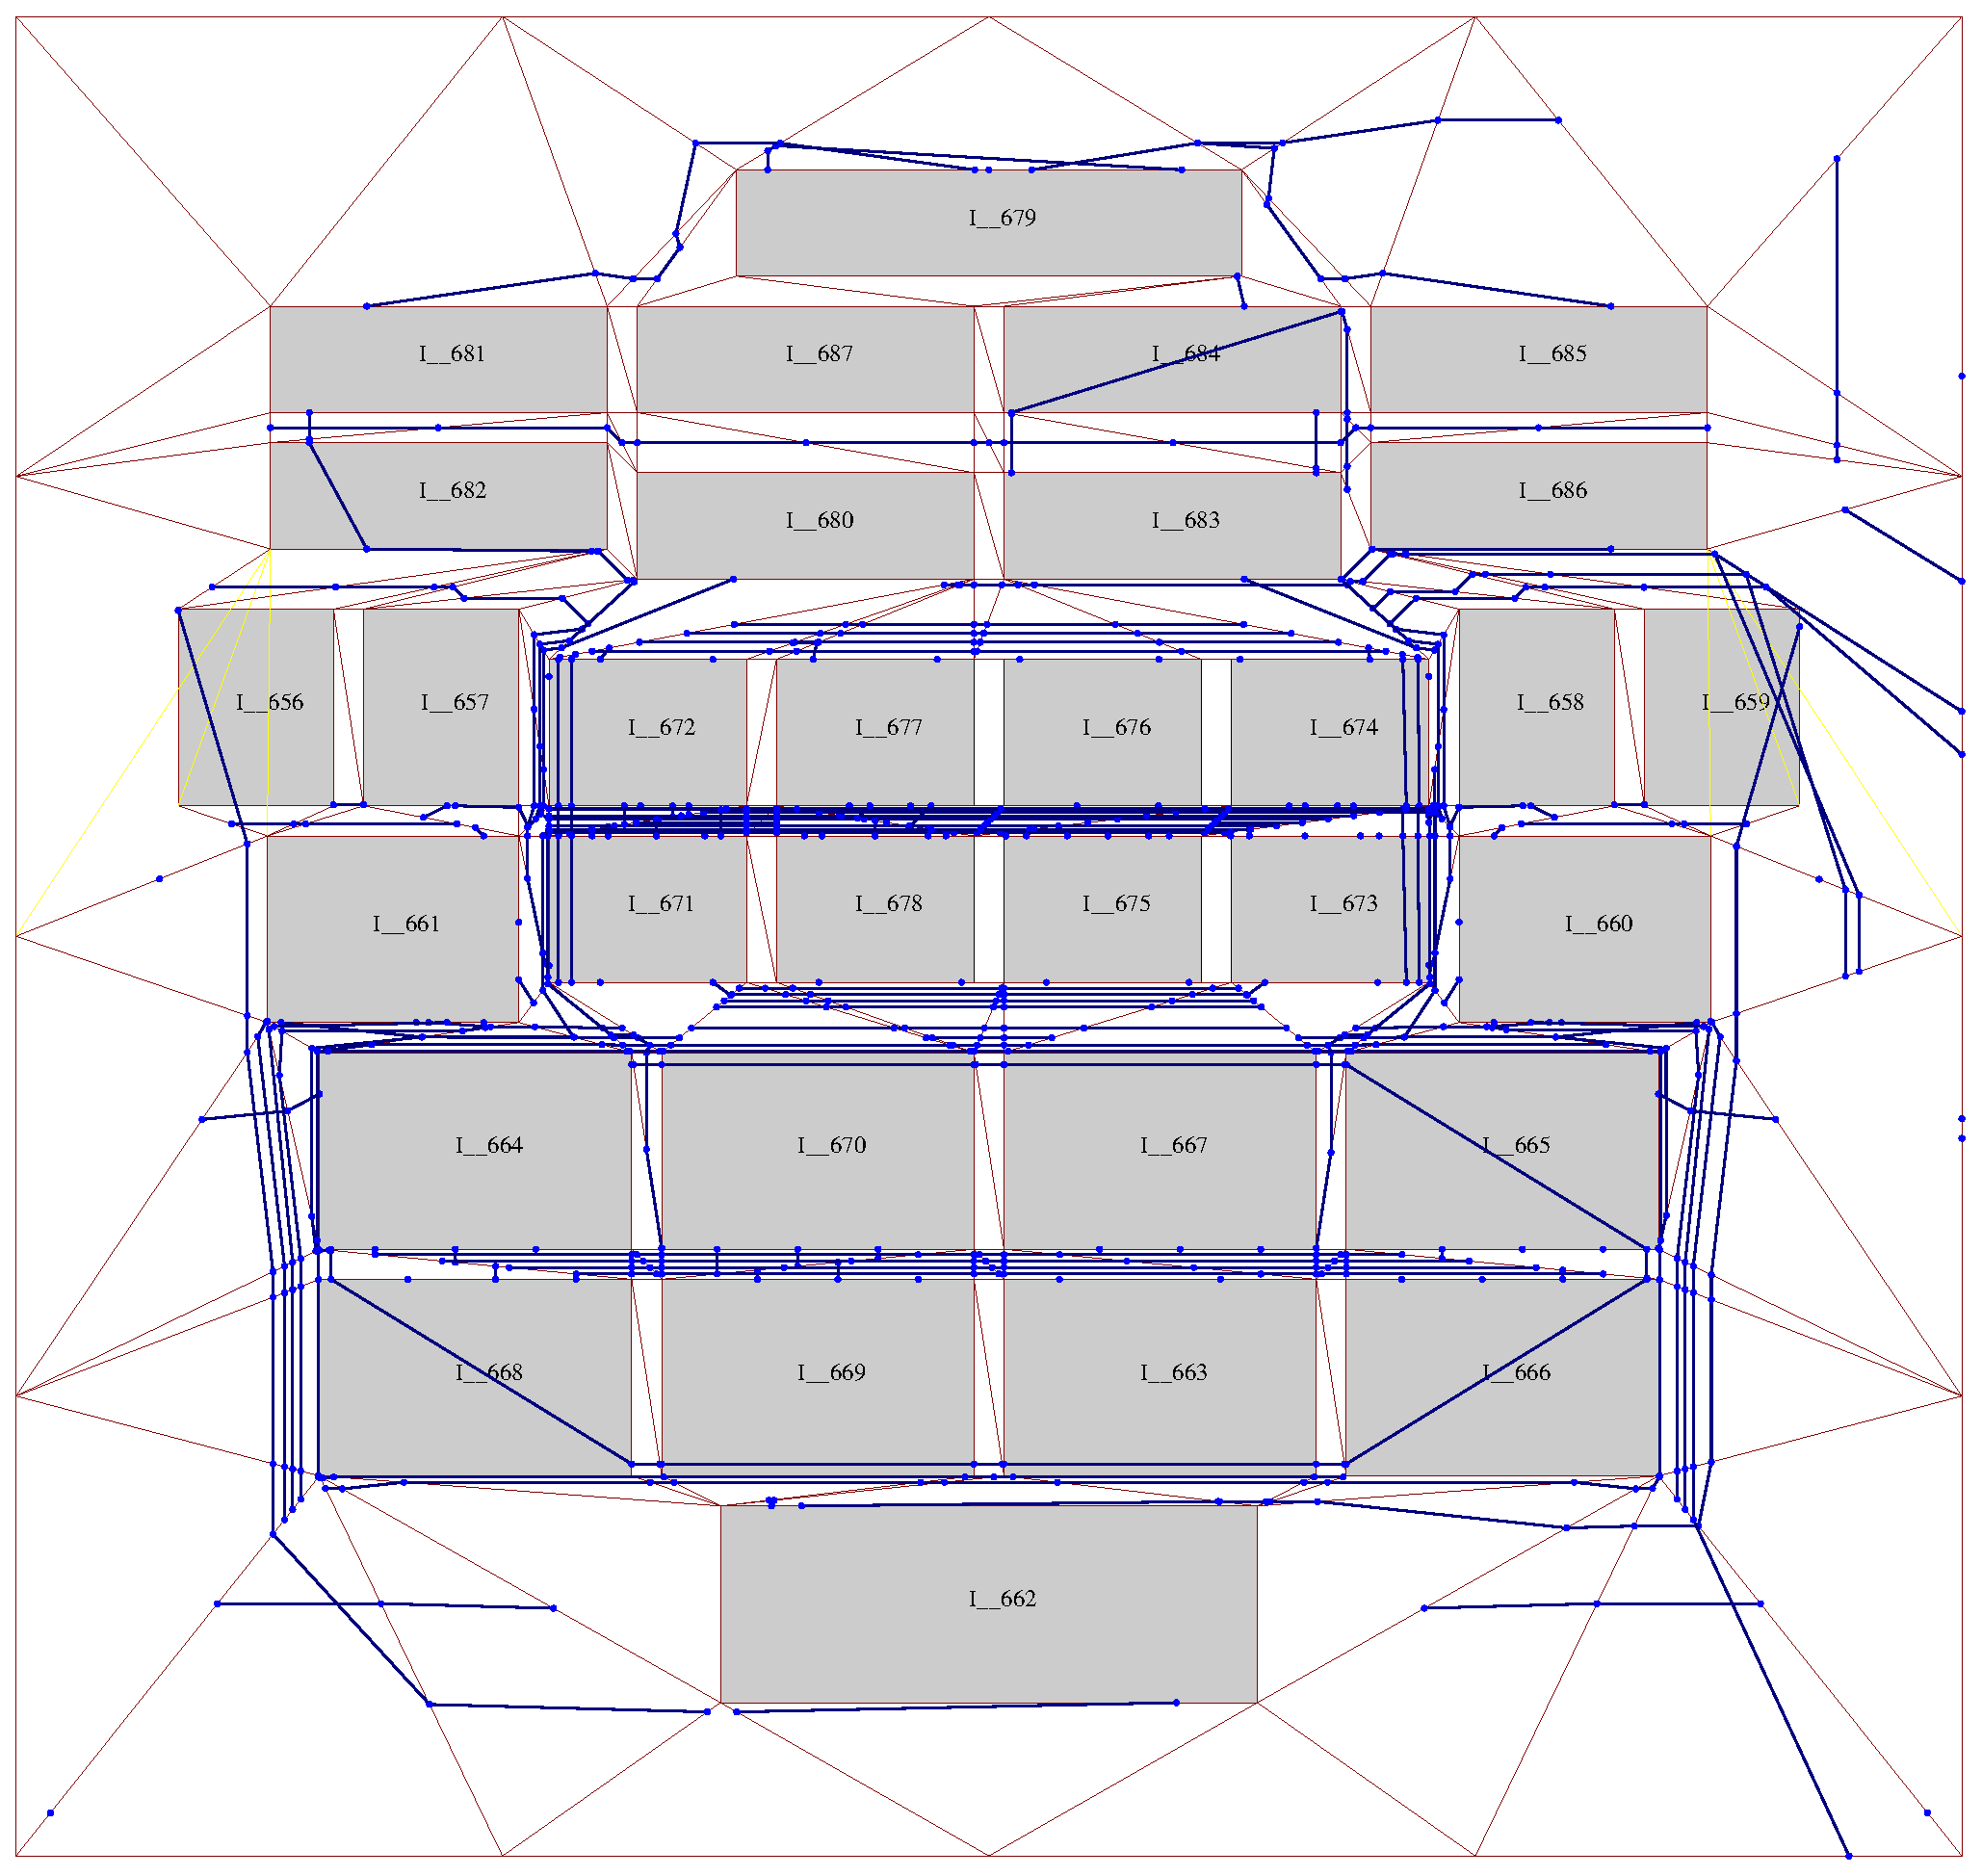
\includegraphics[width=\textwidth]{Fig/VGAProto.eps}
        \caption{VGA umc65nm}\label{fig:VGAProto}
        \end{subfigure}
      \caption{Illustration of crossing graph for OpAmp and VGA before and after updating: (a) extracted crossing graph of OpAmp under umc90nm (b)updated crossing graph under tsmc90nm (c) extracted crossing graph of OpAmp under umc90nm. (d) updated crossing graph of VGA under umc65nm}
      \label{fig:CDTResult}
    \end{figure}

  

  In the third experiment, we further practice original topology with CDT-based migrated routing and our approach on a large multi-level design in Section~\ref{subsec:ExpLDO}. 
  All the experimental results have passed layout verification via DRC, LVS checks, and the simulation data is listed in Table~\ref{table:MigrationPerf}, Table~\ref{table:MultProto} and Table~\ref{table:HierProto}.

  \section{Placement in Original Topology with Different Routing Migrations}\label{sec:ExpMigration}


    First of all, we focus on migrating two circuits based on umc90nm technology to other technology nodes which are umc65nm and tsmc90nm. To reach the requirement of design migration, one circuit should be re-generated on the target technology for the same functionality while satisfying the performance specification. 

    
    
    \begin{table}[ht]
      \hspace{-1em}
      \begin{threeparttable}
      \scriptsize
      \begin{center}
        \caption{Routing Completeness and Performance Comparisons among Migration Targets}\label{table:MigrationPerf}
      \begin{tabular}{|c|c|c|c|c|c|c|c|c|c|c|c|c|}
        \toprule  
        \hline
          \multirow{2}{*}{Circuit}& 
          \multirow{2}{*}{Layout} & 
          \multicolumn{2}{c|}{Overall Routing \tnote{a}} & 
          \multicolumn{2}{c|}{Auto Routing \tnote{b}} & 
          \multicolumn{2}{c|}{Routing Com.\tnote{c} (\%)} & 
          \multirow{2}{1cm}{$A_v$ ($dB$)} & 
          \multirow{2}{1cm}{BW ($MHz$)} & 
          \multirow{2}{1cm}{PM ($deg$)} & 
          \multirow{2}{1cm}{Power ($\mu W$)}  &
          \multirow{2}{*}{Time }\\
          \cline{3-8} 
          & & WL ($\mu m$) & WS \# &  WL ($\mu m$) & WS \#  &  WL ($\mu m$) & WS \# & & & & & \\
        \hline
        %\rowcolor{mygray}
        %\multicolumn{13}{|c|}{OpAmp}\\
        %\hline
        OpAmp:umc90nm &  Origin & 351.438 & & - &-  &-& - & 48.653 &  110.9 & 45.882  & 120.34 &  8 hrs \\
        \hline
        OpAmp:umc65nm &  \cite{msc-bhattacharya-tcad06}+RtMaMi &  321.44 & 38 & - & - & - & - & 43.421& 110.4 &53.294 & 118.66 &  8 hrs \\
        \hline
        OpAmp:umc65nm & \cite{msc-bhattacharya-tcad06}+RtNoMi& 414.84 & 45 & 312.471 & 31 & 75.3\% & 68.89\%& 43.02& 108.6& 56.6& 118.36 &  100 mins \\
        \hline
        OpAmp:umc65nm &  Ours & 298.99& 40 & 231.15 &32 &  77.3 \%& 80.00\% & 43.36 & 110.4 & 56.6 & 118.69 & 40 mins \\
        \hline
        OpAmp:tsmc90nm  &  Ours & 286.954& 38 &  215.204& 33&  74.99 \% & 86.84\%& 45.0 &117.0 &55.9 & 113.3 & 40 mins \\
        %\hline
        %\rowcolor{mygray}
        %\multicolumn{13}{|c|}{VGA}\\
        \hline
        VGA:umc90nm & Origin &  3628.25  &  281& -&-&- & - & 18.48 & 7.237&86.645 & 596.74 & 2 days \\
        \hline
        VGA:umc65nm & \cite{msc-bhattacharya-tcad06}+RtMaMi &  3011.83& 283 & -& - &- & - & 18.57 & 7.427 &90.75& 566.81&   2 days \\
        \hline
        VGA:umc65nm & Ours & 3385.849& 266 &  2877.99& 238 & 85 \% & 89.47\%&18.68 & 7.41& 89.3 & 569.1& 553 mins  \\
        \hline
      \end{tabular}
      \begin{tablenotes}
        \item [a] Overall routing characteristics including the wirelength and the number of wire segments. 
        \item [b] Automatic generated routing characteristics
        \item [c] Routing completeness is the ratio between auto-gen routing and overall routing. 
      \end{tablenotes}
      \end{center}
      \end{threeparttable}
    \end{table} 
       

    Figure~\ref{fig:CDTResult} illustrates the crossing graph generated from template layouts and the updated graph from target layouts. Figure~\ref{fig:OrigOpamp} shows the crossing graph of OpAmp with only one routing path being displayed, and Figure~\ref{fig:OpampProto} shows the updated crossing graph for tsmc90nm. We can find out that the routing behavior is recorded by the graph when the placement is changed. Figure~\ref{fig:OrigVGA} shows one of the crossing graphs of VGA circuit since VGA has more than one hierarchy with all routing paths on it. Figure~\ref{fig:VGAProto} shows the updating graph for umc65nm. Although VGA has much more routing nets than OpAmp, routing behavior of each routing paths is preserved in the crossing graph. The purple points along the routing edges implies the original vertices of wire segments, which are not regarded as crossing vertices, and the blue points are crossing points as mentioned in \ref{sec:CGC}. Figure~\ref{fig:PPL_OPT90} and Figure~\ref{fig:PPL_VGAU65} illustrate the updated crossing graphs of Figure~\ref{fig:ML_OPU90} and Figure~\ref{fig:ML_VGAU90} respectively. The yellow edges are the {\it invalid} crossing edges, after updating. As mentioned in Section~\ref{sec:updateG}, these {\it invalid} crossing edges overlap the blocks after updating.

    \begin{figure}[ht]
      \centering
        \begin{subfigure}[t]{0.4\textwidth}
        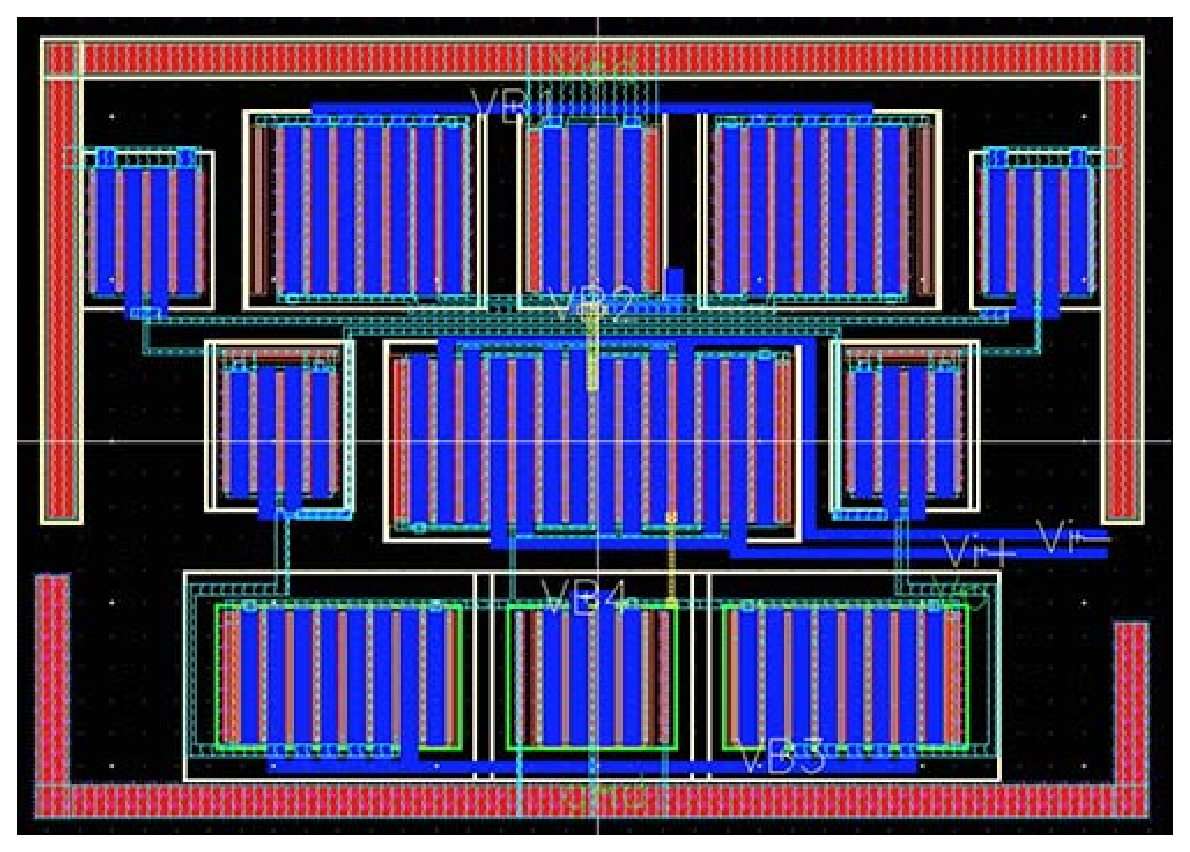
\includegraphics[width=\textwidth]{Fig/ML_OPU90.eps}
        \caption{OpAmp:umc90nm Ori. Layout}\label{fig:ML_OPU90}
        \end{subfigure}
        \begin{subfigure}[t]{0.4\textwidth}
        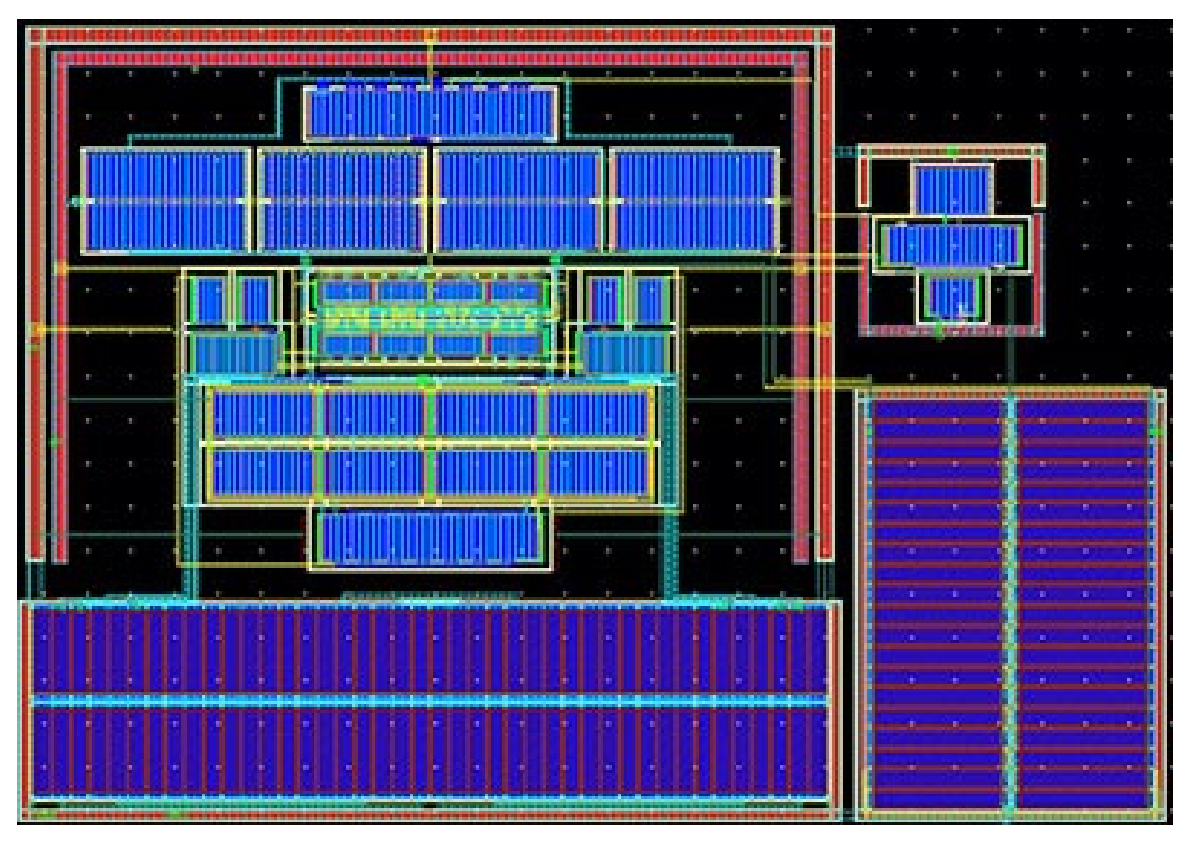
\includegraphics[width=\textwidth]{Fig/ML_VGAU90.eps}
        \caption{VGA:umc90nm Ori. Layout}\label{fig:ML_VGAU90}
        \end{subfigure}
        \begin{subfigure}[t]{0.4\textwidth}
        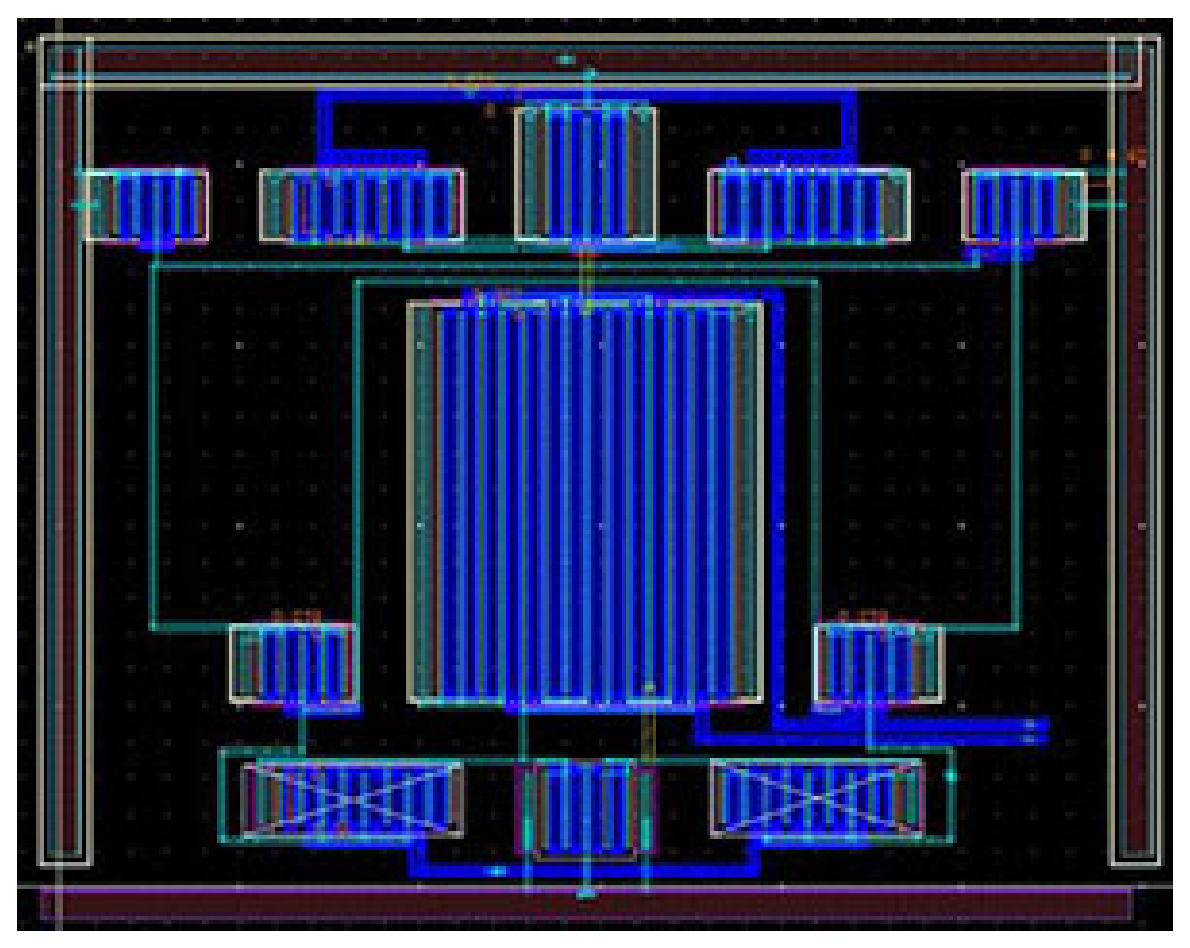
\includegraphics[width=\textwidth]{Fig/PPL_OPT90.eps}
        \caption{OpAmp:tsmc90nm our approach}\label{fig:PPL_OPT90}
        \end{subfigure}
        \begin{subfigure}[t]{0.4\textwidth}
        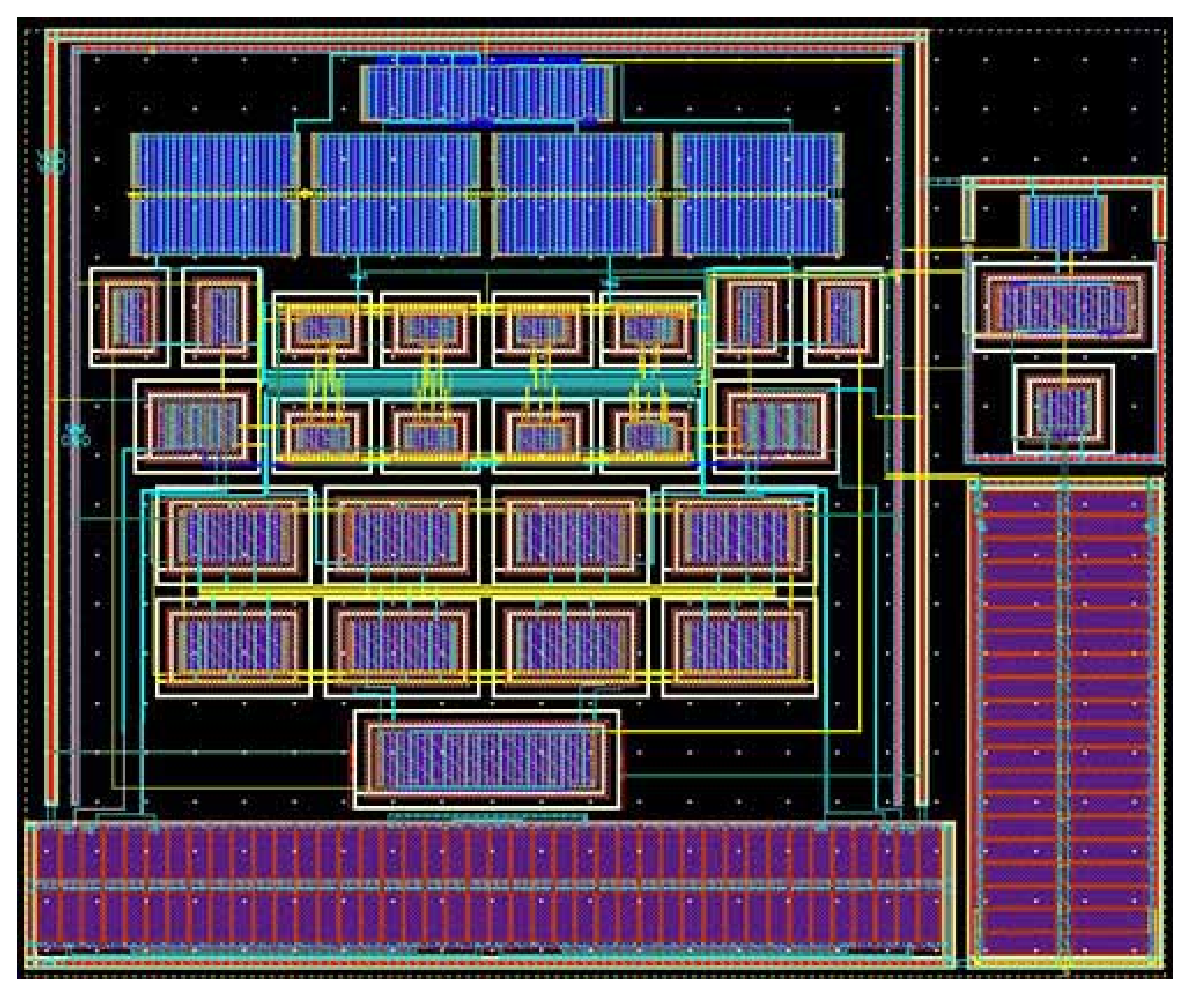
\includegraphics[width=\textwidth]{Fig/PPL_VGAU65.eps}
        \caption{VGA:umc65nm our approach}\label{fig:PPL_VGAU65}
        \end{subfigure}
      \caption{Migration comparison on Op-Amp design among (a) Original layout. (b) Placement fully and routing fully migrated to umc65nm (c) Placement with original topology and routing preserved to umc65nm and (d) Placement with original topology and routing preserved to tsmc90nm.}\label{fig:Layout}
    \end{figure}



    Figure~\ref{fig:Layout} illustrates the layout results of migrated designs. Figure~\ref{fig:ML_OPU90} and Figure~\ref{fig:ML_VGAU90} illustrates the original layouts of OpAmp and VGA respectively. Figure~\ref{fig:PPL_OPT90} gives the migrated results obtained by our methodology under tsmc90nm technology. It is easy to observe that even though placement is changed due to different block size, the routing correlation with placement is preserved under tsmc90nm technology. Figure~\ref{fig:PPL_VGAU65} illustrates the migrated VGA under umc65nm. Since there are three common-centroid structures in the VGA layout, more wires are connected inside these common-centroid structures. While RtMaMi takes time to re-construct the routing in manual, the crossing graph can migrate the relative location for these wires in a flexible manner.


    Based on migrated placement by \cite{msc-bhattacharya-tcad06} and our approach, there are three migration strategies performed towards OpAmp and VGA design under different technologies. These are RtMaMi, RtNoMi and our approach. Table~\ref{table:MigrationPerf} records the wirelength, the number of wire segments and the simulation data. We compare the overall routing WL, automatically generated WL and the routing completeness on wirelength firstly. The overall wirelength consists of wires by manual automated routing. Since circuit sizing in umc65nm can be scaled down to satisfy performance specifications, the devices' size and WL are proportionally smaller as well. The routing completeness of WL is expressed as the ratio between auto-generated routing over total wirelength. However, the distance between blocks are diverse to measure the routing completeness with wirelength is not comprehensive. Therefore, we also consider the re-coverage of wire segment (WS). The routing completeness of WS implies how many essential wire segments is automatically generated by program. Obviously, even though RtNoMi generates routing result automatically, it still takes time to refine the layout for accuracy. We can see the routing completeness of RtNoMi are 75.3\% and 68.9\% for WL and WS respectively. We can tell that, most of the RtNoMi results in the OpAmp circuit are failed with LVS checking so that it leaves part of wire in manual refinement.

    \begin{figure}[ht]
      \centering
      \begin{subfigure}[t]{0.2\textwidth}
      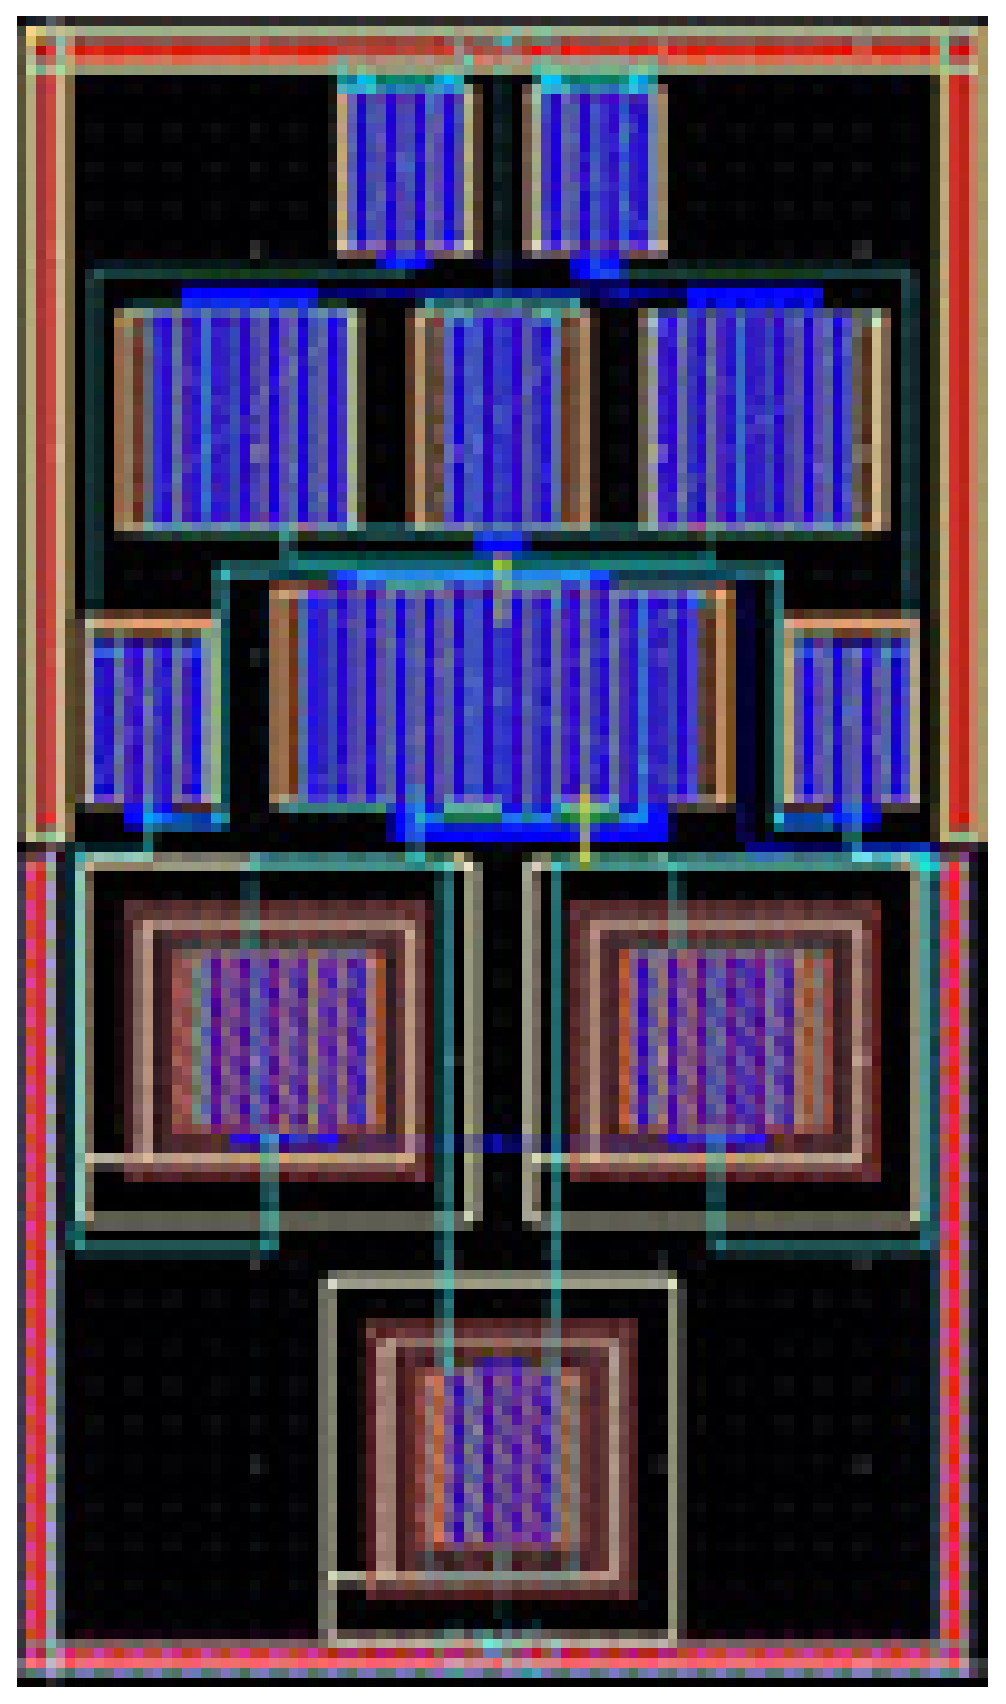
\includegraphics[width=\textwidth]{Fig/MultTopo_Topo2.eps}
      \caption{Topo2}\label{fig:Topo2}
      \end{subfigure}
      \begin{subfigure}[t]{0.2\textwidth}
      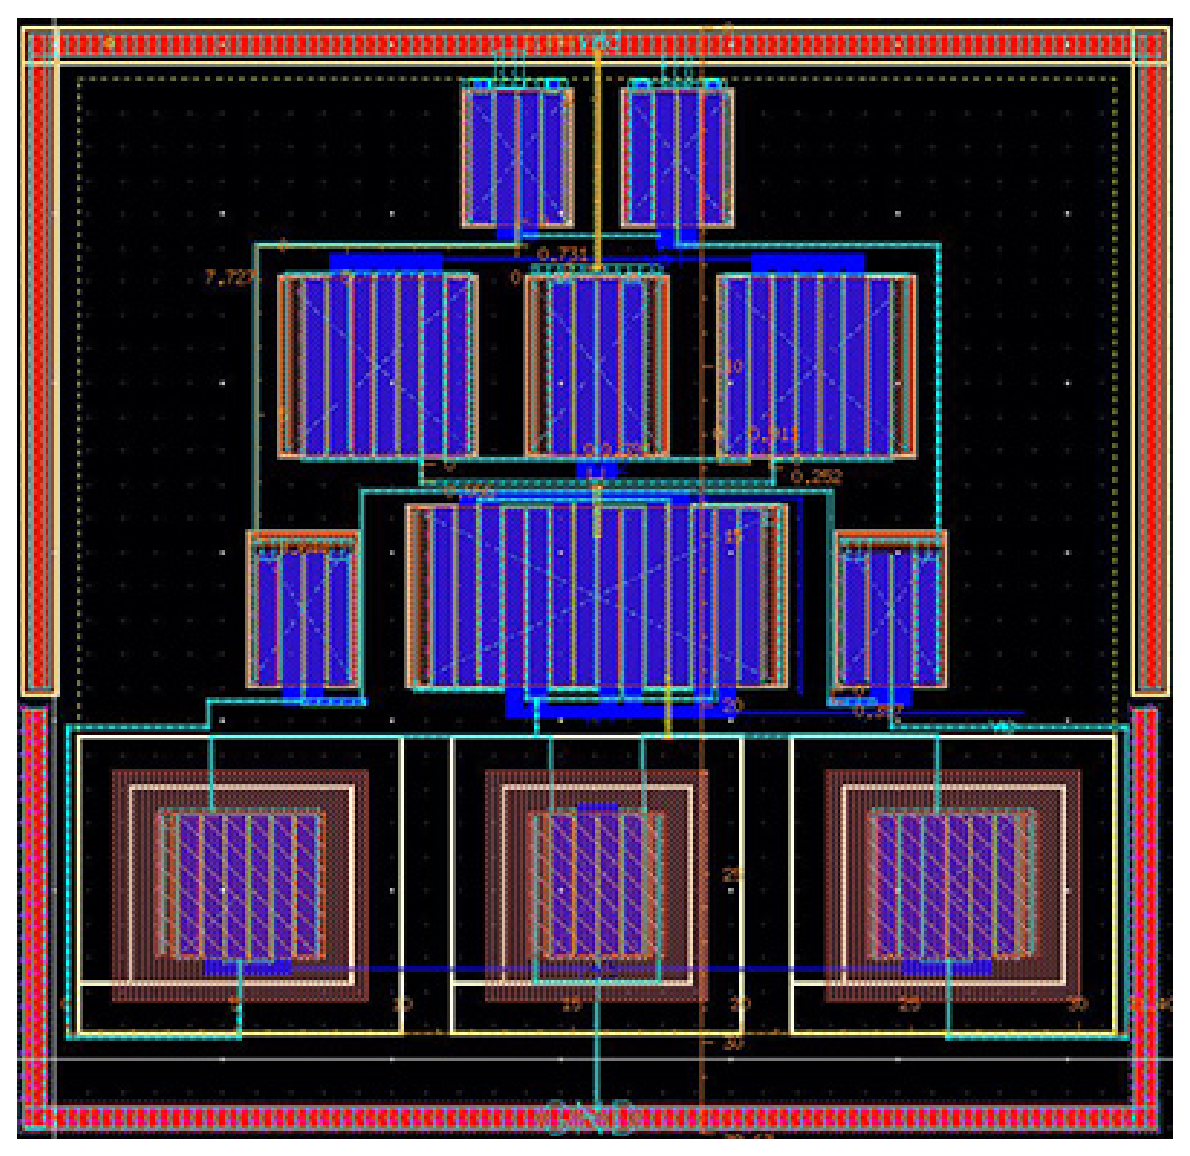
\includegraphics[width=\textwidth]{Fig/MultTopo_Topo3.eps}
      \caption{Topo3}\label{fig:Topo3}
      \end{subfigure}
      \begin{subfigure}[t]{0.2\textwidth}
      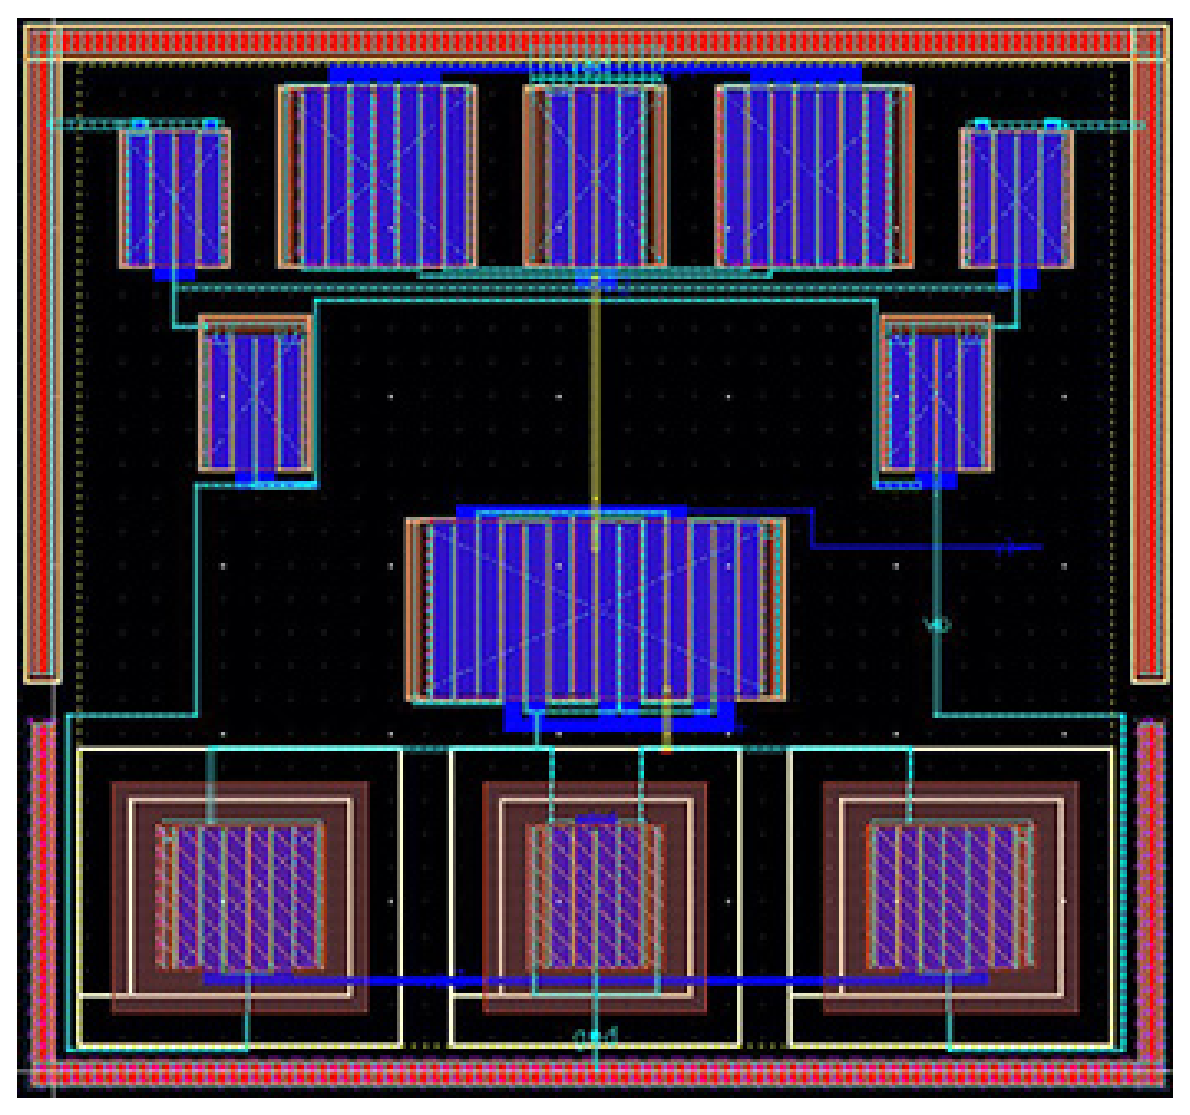
\includegraphics[width=\textwidth]{Fig/MultTopo_Topo4.eps}
      \caption{Topo4}\label{fig:Topo4}
      \end{subfigure}
      \begin{subfigure}[t]{0.2\textwidth}
      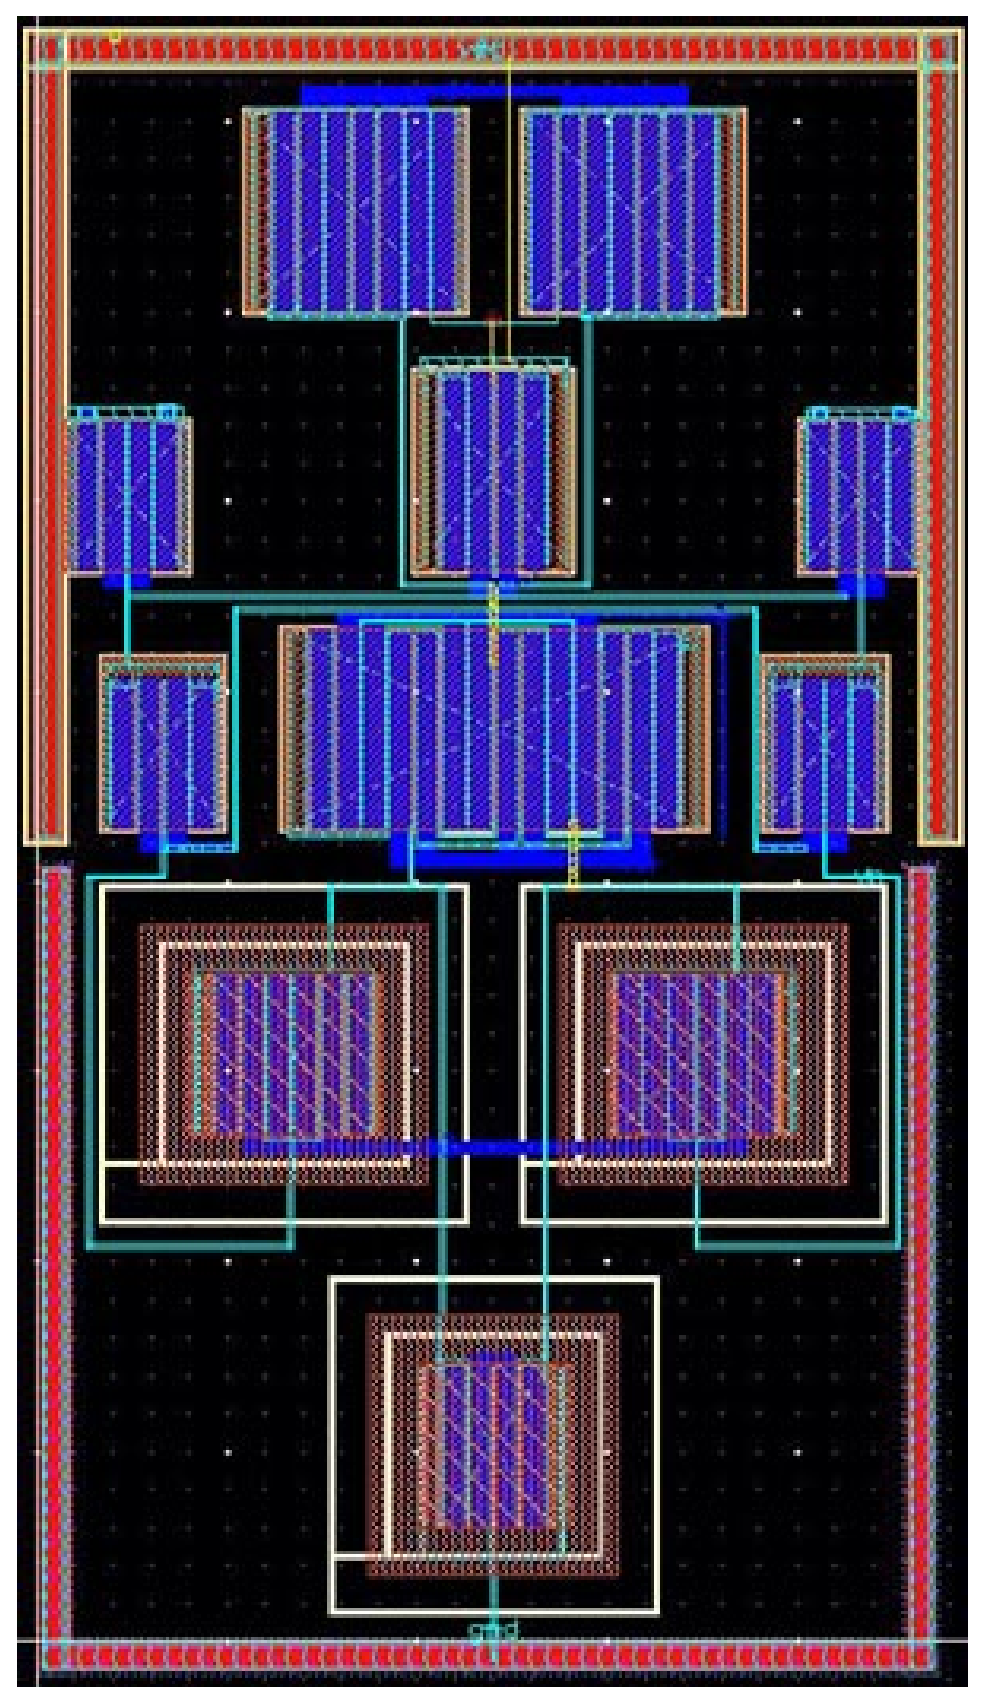
\includegraphics[width=\textwidth]{Fig/MultTopo_Topo5.eps}
      \caption{Topo5}\label{fig:Topo5}
      \end{subfigure}
      \begin{subfigure}[t]{0.2\textwidth}
      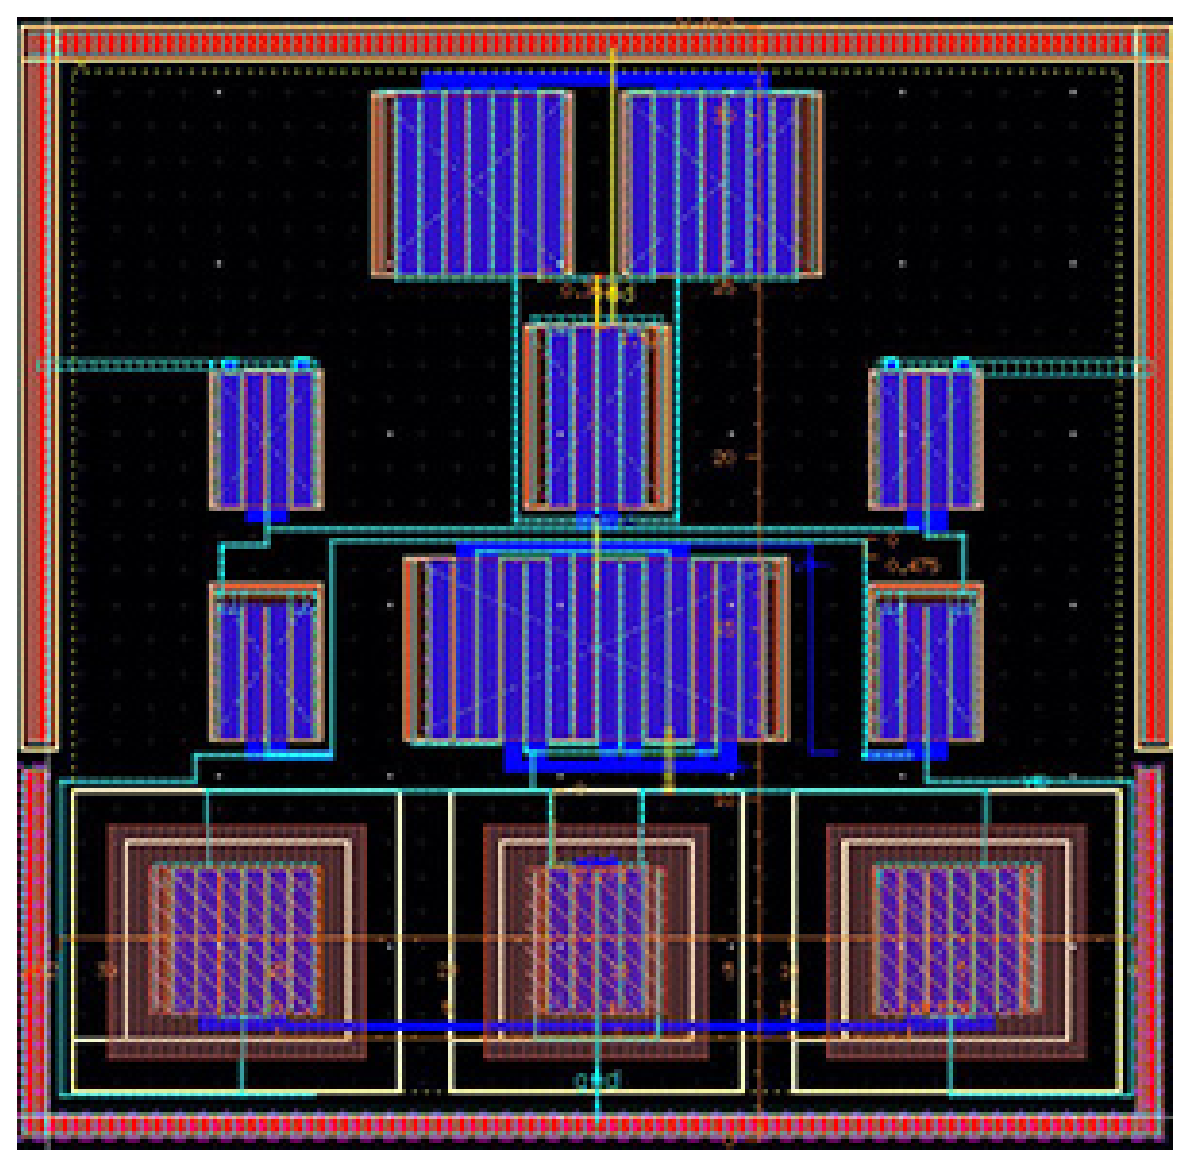
\includegraphics[width=\textwidth]{Fig/MultTopo_Topo6.eps}
      \caption{Topo6}\label{fig:Topo6}
      \end{subfigure}
      \begin{subfigure}[t]{0.2\textwidth}
      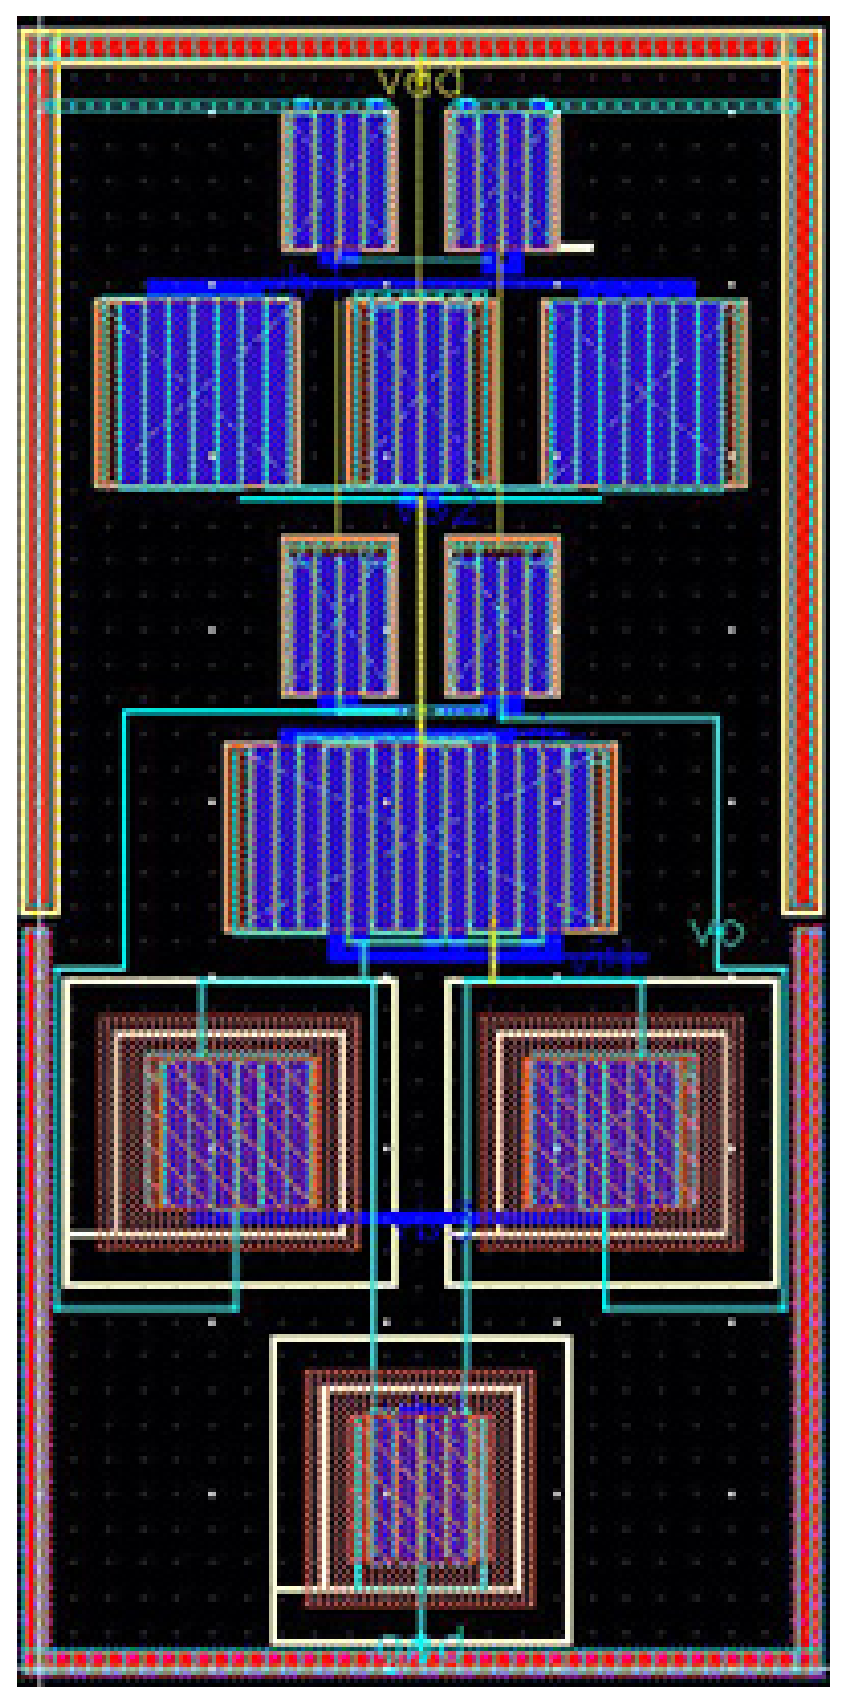
\includegraphics[width=\textwidth]{Fig/MultTopo_Topo7.eps}
      \caption{Topo7}\label{fig:Topo7}
      \end{subfigure}
      \begin{subfigure}[t]{0.2\textwidth}
      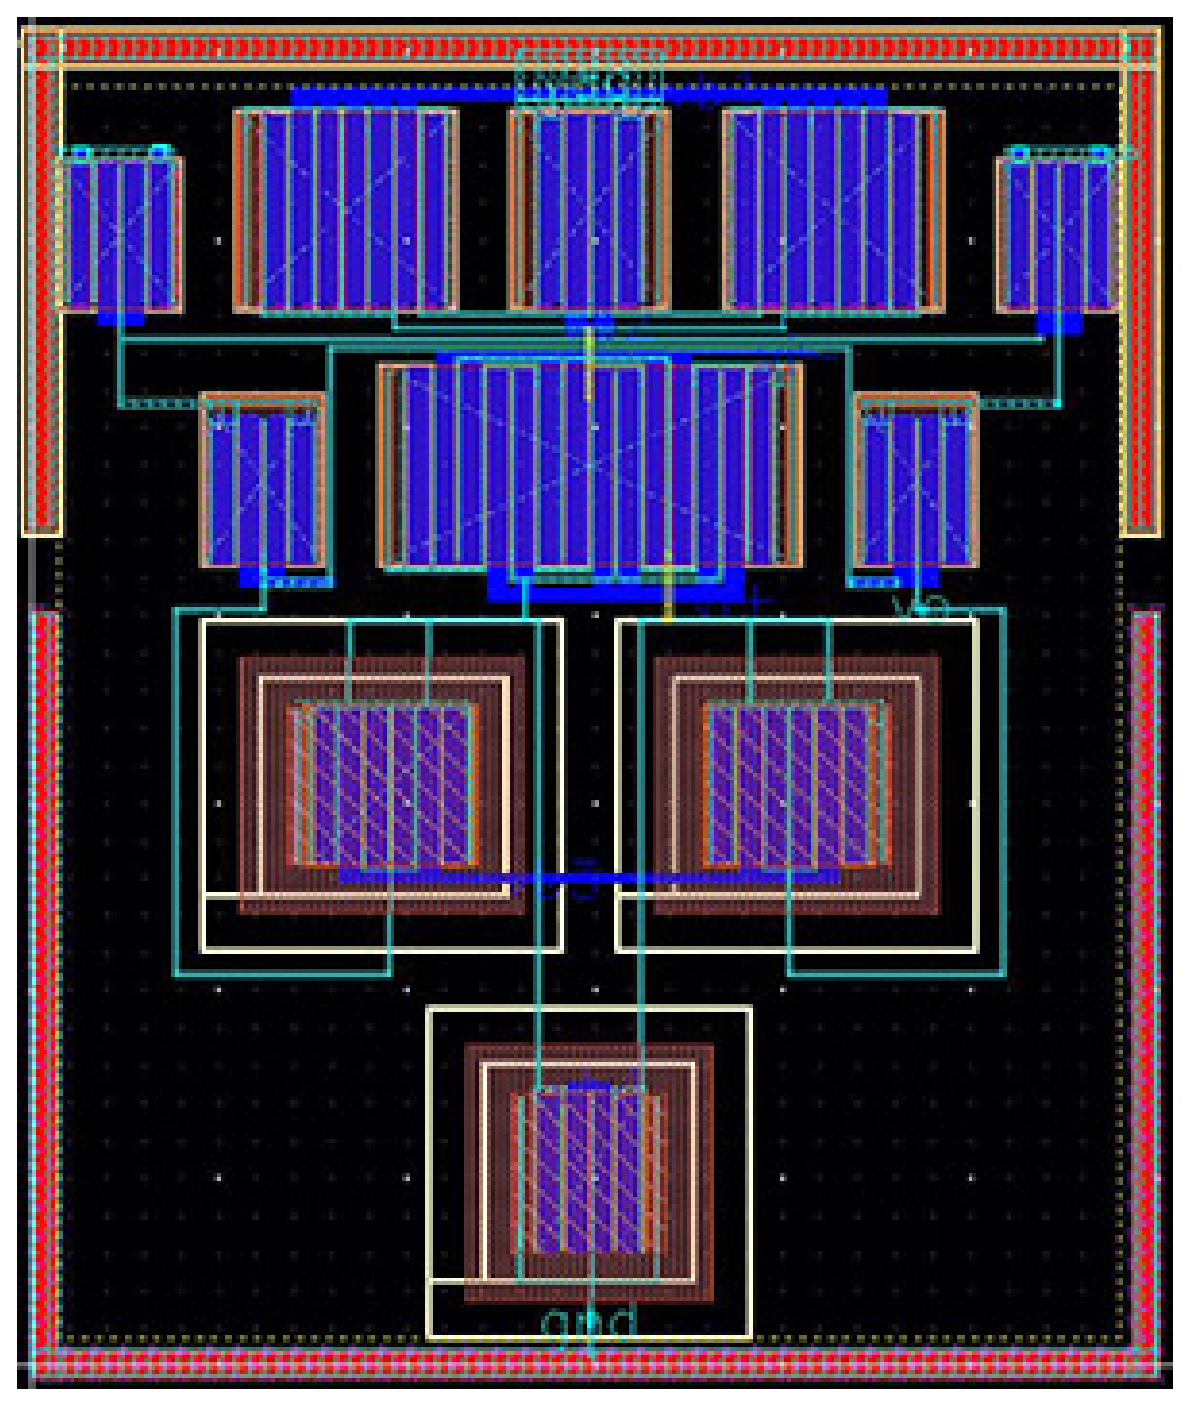
\includegraphics[width=\textwidth]{Fig/MultTopo_Topo8.eps}
      \caption{Topo8}\label{fig:Topo8}
      \end{subfigure}
      \caption{Multiple prototype of layouts achieved by our approach with 7 topologies respectively.}
      \label{fig:MultTopo}
    \end{figure}

    \begin{table}
      \scriptsize
      \begin{center}
        \caption{Routing Completeness and Performance Comparisons among Multiple Migrated Placements}\label{table:MultProto}
        \begin{tabular}{|c|c|c|c|c|c|c|c|c|c|c|c|}
          \toprule
          \hline
          \multirow{2}{*}{Placement}& 
          \multirow{2}{*}{Routing} & 
          \multicolumn{2}{c|}{Overall Routing}  & 
          \multicolumn{2}{c|}{Auto Routing } & 
          \multicolumn{2}{c|}{Routing Com. (\%)} & 
          \multirow{2}{1cm}{\scriptsize $A_v$/$A_v^{WSR}$ ($dB$)} & 
          \multirow{2}{1.3cm}{\tiny $BW$/$BW^{WSR}$ ($MHz$)} & 
          \multirow{2}{1.3cm}{\tiny $PM$/$PM^{WSR}$ ($deg$)} & 
          \multirow{2}{*}{Time}\\
          \cline{3-8} 
          & & WL ($\mu m$) & WS \#  &  WL ($\mu m$) & WS \# &  WL & WS \# & & & & \\
          \hline
            Original Topo. & \multirow{8}{*}{RtMaMi} & 321.44 & 38 &\multirow{8}{*}{-} & \multirow{8}{*}{-} & \multirow{8}{*}{-} & \multirow{8}{*}{-} & 43.421/- & 110.4/- & 53.29/- & 8 hrs \\ \cline{1-1} \cline{3-4} \cline{9-12}
            \cite{ALP_YPWeng_iccad2011}:Topo2 & & 210.53 & 34 & & & & & 43.398/- & 111.22/- & 53.723/- & 3 hrs \\ 
            \cite{ALP_YPWeng_iccad2011}:Topo3 & & 203.2 & 33 & & & & & 43.398/- & 110.63/- & 53.601/- & 3 hrs \\ 
            \cite{ALP_YPWeng_iccad2011}:Topo4 & & 206.625 & 34 & & & & & 43.41/- & 111/- & 53.669/- & 3 hrs \\ 
            \cite{ALP_YPWeng_iccad2011}:Topo5 & & 228.519 & 39 & & & & & 43.393/- & 111/- & 53.617/- & 3 hrs \\ 
            \cite{ALP_YPWeng_iccad2011}:Topo6 & & 274.525 & 38 & & & & & 43.393/- & 110.56/- & 53.496/- & 3 hrs \\ 
            \cite{ALP_YPWeng_iccad2011}:Topo7 & & 226.495 & 32 & & & & & 43.398/- & 111.59/- & 53.917/- & 3 hrs \\ 
            \cite{ALP_YPWeng_iccad2011}:Topo8 & & 238.28 & 36 & & & & & 43.422/- & 110.98/- & 53.412/- & 3 hrs \\
          \hline
            Original Topo. & \multirow{8}{*}{RtNoMi} & 414.84 & 45 & 312.471 & 31 & 75.3\% & 68.89\% & 43.02/- & 108.6/- & 56.6/- & 100 mins \\ \cline{1-1} \cline{3-12}
            \cite{ALP_YPWeng_iccad2011}:Topo2 & & 401.896 & 48 & 316.8 & 37 & 78.8\% & 77.08\% & 42.69/- & 112.8/- & 57.57/- & 60 mins \\
            \cite{ALP_YPWeng_iccad2011}:Topo3 & & 392.777 & 45 & 311.2 & 35 & 79.23\% & 77.78\% & 42.99/- & 109.3/- & 57.35/- & 40 mins \\
            \cite{ALP_YPWeng_iccad2011}:Topo4 & & 486.795 & 47 & 369.3 & 34 & 78.86\% & 72.34\% & 43.03/- & 108.2/- & 57.3/- & 35 mins \\
            \cite{ALP_YPWeng_iccad2011}:Topo5 & & 395.9 & 44 & 316.6 & 36 & 79.97\% & 81.82\% & 42.74/- & 108.6/- & 57.71/- & 1 hrs \\
            \cite{ALP_YPWeng_iccad2011}:Topo6 & & 408.7 & 46 & 316.8 & 34 & 77.51\% & 73.91\% & 42.75/- & 108.8/- & 57.34/- & 65 mins\\
            \cite{ALP_YPWeng_iccad2011}:Topo7 & & 406.55 & 44 & 298.1 & 32 & 73.32\% & 72.73\% & 42.98/- & 109.6/- & 57.7/- & 43 mins \\
            \cite{ALP_YPWeng_iccad2011}:Topo8 & & 435.56 & 41 & 334.7 & 33 & 76.84\% & 80.49\% & 42.77/- & 108.7/- & 57.54/- & 45 mins \\
          \hline
            Original Topo. & \multirow{8}{*}{Ours} & 298.99 & 40 & 231.15 & 32 & 77.31\% & 80\% & 43.348/43.36 & 110.37/110.4 & 56.6/56.6 & 42 mins \\ \cline{1-1} \cline{3-12}
            Ours:Topo2 & & 275.569 & 38 & 204.176 & 31 & 79.27\% & 81.58\% & 43.388/43.42 & 109.6/109.0 & 49.3/50.7  &  41 mins \\
            Ours:Topo3 & & 278.023 & 43 & 232.866 & 35 & 83.7\% & 81.4\% &  43.41/43.431 & 109.8/110.2 & 55.6/55.6 & 31 mins \\
            Ours:Topo4 & & 307.136 & 44 & 280.72 & 35 & 91.4\% & 79.55\% & 43.407/43.412 & 108.9/109.3 & 51.0/51.0 &  28 mins \\
            Ours:Topo5 & & 255.039 & 41 & 218.624 & 35 & 85.7\% & 85.37\% & 43.38/43.4&  110.3/110.1 & 54.8/54.8 & 36 mins \\
            Ours:Topo6 & & 291.645 & 45 & 249.964 & 38 & 85.7\% & 84.44\% &  43.40/43.41 &  109.8/109.8 & 54.3/54.3 & 31 mins \\
            Ours:Topo7 & & 235.406 & 39 & 191.538 & 30 & 81.4\% & 76.92\% &  43.386/43.41&  110.2/110.8 &  55.4/55.3 &  26 mins \\
            Ours:Topo8 & & 265.898 & 43 & 238.07 & 37 & 89.5\% & 86.05\% &  43.408/43.42 &  110.3/110.7 & 54.9/ 54.9 &  29 mins \\
          \hline
            \multirow{3}{1.5cm}{Normalized  Comparison} & 
              RtMaMi    & 1 & 1 &- &- & - & - &  1 & 1.02 &  0.99 & 8.7  \\
              \cline{2-12}
              & RtNoMi  & 1.75  & 1.27 & 1.39 &  1.01 & 0.92 & 0.94 & 0.988 & 1.005 &  1.06 & 1.99   \\
              \cline{2-12}
              & Ours    & {1.16}  & 1.17 & 1    & 1   &  1  & 1 &  1 &  1 & 1 &  1 \\
          \hline

        \end{tabular}
        %\begin{tablenotes}
        %  \item [a] $A_v^{WSR}$ denotes the voltage gain performance after implementing {\it Wire %Segment Refinement.}
        %  \item [b] $BW^{WSR}$ denotes the bandwidth performance after implementing {\it Wire Segment %Refinement.}
        %  \item [C] $PM^{WSR}$ denotes the phase margin performance after implementing {\it Wire Segment %Refinement.}
        %\end{tablenotes}
      \end{center}
      %\end{threeparttable}
    \end{table}

    In average, our approach obtains routing completeness on WL more than 75\% in OpAmp case and 85\% in VGA case. The characteristics on WS are even better: 80\% routing completeness for OpAmp on umc65nm and 86.8\% on tsmc90nm. Still, our approach earns 89.47\% WS for VGA. The more routing completeness for routing, the less wire needed to be refined. Considering design time for these routing strategies, it includes routing generation, detailed routing refinement and physical verification as a complete layout generation flow. RtMaMi takes most of the time on layout design manually. On the other hand, RtNoMi and our approach apply routing algorithms to automatically generate an rough routing result. Therefore, we tend to illustrate the giant differentiation among manual routing and automatic routing via design time comparison. In OpAmp case, both umc90nm and umc65nm take 8 hrs to complete the routing, and VGA takes 2 days for RtMaMi in both technologies. RtNoMi is faster than RtMaMi with 100 minutes design time. Other than RtMaMi and RtNoMi, our approach only takes 30 minutes to strive the complete layout. As a result, our approach which demonstrates the efficiency in timing issue, represents an effective routing recovering strategy on migration. 

    Also, we compare the performance for voltage gain ($A_v$), bandwidth (BW), phase margin (PM), power consumption (Power) and design time in the right part of Table~\ref{table:MigrationPerf}. In OpAmp case, RtMaMi earns the first place of voltage gain $A_v$. However, our approach obtains better $A_v$ than the others under umc65nm. Meanwhile, our method also acquires better performance for $A_v$, BW and Power under tsmc90nm. In VGA case, we consider RtMaMi and our approach for migration under umc65nm, and our approach obtains better performance than RtMaMi. Hence, as a prove for Table~\ref{table:MigrateComp}, our approach is obviously faster than \cite{msc-bhattacharya-tcad06}+RtMaMi because routing can be generated efficiently with CDT preservation. Also, the higher routing completeness of our approach than RtNoMi's results in better runtime.


  \section{Multiple Placement Solutions with Different Routing Migrations}\label{sec:ExpMultiProto}

    %In previous subsection, the migration is implemented in the original topology of placement with different routing strategies. 
    In this section, multiple topologies of placement with aforementioned routing approaches are practiced. Our experiments are performed with OpAmp under umc65nm technology. 
    %To avoid process variation damaging performance of analog design, analog placement should take care of several placement constraints, such as symmetry and matching constraints. In the experiments of \cite{ALP_YPWeng_iccad2011}, multiple placement topologies are generated considering these constraints. 
    We extend the experiment in \cite{Chin_DMR_ICCAD2013} with different routing migration skill. Furthermore, the comparison among performance before and after {\it Wire Segment Refinement} is also delivered. This experiment aims to show the flexibility of placement topology, the completeness of our routing approach and the effectiveness of wire refinement method.

    Figure~\ref{fig:MultTopo} illustrates seven prototypes with our prototyping technique. Table~\ref{table:MultProto} displays the results of different migrated placements with RtMaMi, RtNoMi and our approach, respectively. The resulting data includes wirelength (WL), number of wire segments (WS \#), performance and timing. Different migrated placements result in different routing behaviors and different performances obviously. According to the RtMaMi results, \cite{ALP_YPWeng_iccad2011}:Topo8 earns better routing result and performance than Original Topology. For the same routing strategy, Table~\ref{table:MultProto} represents the possibility with different placement topologies. On the other hand, we can see most of the results of RtNoMi are worse than RtMaMi among different migrated placements. In addition, the routing results and performance of our approach are better that RtNoMi among these migrated placements. 

    As introduced in Section~\ref{chap:WireSegRefine}, {\it Wire Segment Refinement} (WSR) searches for better solution with widening the width of wires. Table~\ref{table:MultProto} also provides the performance before and after WSR. WSR is only implemented in our approach. Therefore, performance metrics like $A_v^{WSR}$, $BW^{WSR}$ and $PM^{WSR}$ represent the performance after WSR. $A_v^{WSR}$ earns better performance than $A_v$ in every Topology. Furthermore, our approach with WSR obtains slightly better performance than RtNoMi in every topology.

    To observe the average performance of each routing migrated techniques, eight migrated placements' results are normalized in the bottom of Table~\ref{table:MultProto}. For the overall routing results, we can observe that our approach is closer to the RtMaMi's result than RtNoMi with WL and WS. According to the auto routing part, our approach obtains better routing completeness than RtNoMi both in WL and WS. For the circuit performance, $A_v$ and $BW$ of our approach are better than RtNoMi. Likewise, the runtime of our approach earns 8.7x and 2x times faster than RtMaMi and RtNoMi, respectively. 

    Moreover, for the same migrated placement, our approach also represents better routing completeness with WL and the WS. From this experiment, we briefly summarize two major idea. First of all, placement with multiple prototypes provides more opportunities on the targeting technology, which can be verified on different routing migrated techniques. Second, our approach generates multiple solutions as \cite{ALP_YPWeng_iccad2011} and reduces time-to-sign-off with routing preservation, and gains better performance with WSR. 

    %Overall, $A_v$ of preserved routing are better than non-preserved in all case of topologies. For bandwidth, preserved routing performs better than non-preserved routing in all cases except Topo2. On the other hand, we investigate that PM of preserved routing is averagely 3.43({\it deg}) worse than non-preserved style. Nevertheless, such quantity of difference in PM affects few towards circuit stability. While non-preserved routing obtains better PM performance, other performances are worse than manual routing and preserved routing. 

    %We can tell that preserved behavior acquires better solution than non-preserved behavior and is comparable to manual style. Preserved approach takes less than half hour to produce layouts in all cases of topologies. Meanwhile, non-preserved technique needs more design time to correct the layout result and it obtains less routing completeness in every prototypes than preserved routing. Both WL and WS are 0.92x of routing completeness with normalized comparison, but the design time of non-preserved design raises up to almost 2x longer than preserved method. It implies that our preservation for routing have kept the advantage of original design for voltage gain, bandwidth, routing completeness and time-to-fabricate. 

    %\begin{figure}[t]
    %  \centering
    %  \epsfig{file=Fig/LDO_chart.eps,width=8cm}
    %  \caption{Schematic structure of LDO. \cite{ERRAmp_LDO,LDO_JSSC,BANDGAP_ICM2010}}
    %  \label{fig:LDO_chart}
    %\end{figure}


    \begin{table}[ht]
      \scriptsize
      \begin{center}
        \caption{Total modules and devices of LDO}\label{table:NumDeviceofLDO}
        \begin{tabular}{|c|c|c|}
        \toprule
        \hline
        Module Name &  Sub-modules or Devices & Total Device \# \\
        \hline
        Bandgap &  \tabincell{c}{Bias + Two-stage \\+ 3MOS + 2BJT+ 13Res} &  37\\
        \hline
        Bias  & 6MOS + 3Res & 9 \\
        \hline
        Driver & \tabincell{c}{Two-stage-OP\\ + Pass-Device\\ + Feedback} & 14\\
        \hline
        Pass-Device & 1 MOS & 1 \\
        \hline
        Feedback & 3 Res & 3\\
        \hline
        Two-stage-OP & 8MOS + 1Res + 1Cap & 10\\
        \hline
        LDO  & Bandgap + Driver & 51\\
        \hline
        \end{tabular}
      \end{center}
    \end{table}


  \subsection{Different Placement Migration with CDT-based Routing Migration}\label{subsec:ExpLDO}

    %For the purpose of understanding the reusability of the hierarchical prototyping from Section~\ref{sec:prototyping}, we have practiced further statistics on a multi-level design, low drop-out regulator (LDO). 
    We practice our approach on a multi-level design, low drop-out regulator (LDO) in this section. For the LDO composition in Table~\ref{table:NumDeviceofLDO}, the overall number of devices of LDO is 51, which can be partitioned into 2 sub-modules: Bandgap and Driver. Both apply the same two-stage-OP as components for reusability, and the deepest level of LDO design is 3.

    

    

    \newcolumntype{P}[1]{>{\RaggedRight\hspace{0pt}}p{#1}}
    \begin{table}[ht]
      \scriptsize
      \begin{center}
        \caption{Comparison on LDO Layout via \cite{msc-bhattacharya-tcad06}+\cite{Chin_DMR_ICCAD2013} and ours on hierarchical prototyping with tsmc90nm, umc90nm and umc65nm}\label{table:HierProto}

        \begin{tabular}{|c|c|c|c|c|c|c|}
          \toprule
          \hline 
          \multirow{2}{*}{Performance}&\multirow{2}{*}{Specification} & tsmc90nm & \multicolumn{2}{c|}{umc90nm}& \multicolumn{2}{c|}{umc65nm} \\
          \cline{3-7}
            & &  Origin & \cite{msc-bhattacharya-tcad06}+\cite{Chin_DMR_ICCAD2013} & Our approach & \cite{msc-bhattacharya-tcad06}+\cite{Chin_DMR_ICCAD2013} & Our approach\\
          \hline
          Minimum input voltage  & 1.1V & 1.1V & 1.1V & 1.1V& 1.1V& 1.1V \\
          \hline
          Nominal output voltage & 1.0V & 1.019 $\sim$ 1.00184V & 1.016 $\sim$ 1.0129V & $1.019 \sim 1.051V$ & 1.0128 $\sim$ 1.0101V & $1.0122 \sim 1.0095V$\\
          \hline
          Dropout voltage & 100 $mV$ & 80.5 $\sim 81.6mV$ & $84 \sim 87.1mV$ & $80.1 \sim 84.9mV$ & $87.2\sim 89.9mV$ & $87.8\sim 90.5mV$ \\
          \hline
          Maximum load current & 50$mA$ & 50$mA$ & 50$mA$ & 50$mA$ & 50$mA$ & 50$mA$ \\
          \hline
          Quiescent current & $\leq1000 \mu A$ & $311\mu A$ & $685\mu A$ & $510.5\mu A$ & $844.1\mu A$ & $809.2\mu A$ \\
          \hline
          Minimum $R_{on}$($@I_{max}$) & $1 \sim 3 \Omega$ & $1.632\Omega$ & $1.682\Omega$  & $1.858\Omega$ & $1.744\Omega$ & $1.81\Omega$ \\
          \hline
          $V_{out}$ Settling time($V_{dd}=1.1V$) & $10\mu S$ & $4.6\mu S$ & $7.4\mu S$& $7.06\mu S$ & $3.2\mu S$ & $3.1\mu S$ \\
          \hline
          Temperature($I_{max}@50mA$) & 100ppm/$\,^{\circ}\mathrm{C}$ &  141ppm/$\,^{\circ}\mathrm{C}$ &  82.6ppm/$\,^{\circ}\mathrm{C}$ &  92ppm/$\,^{\circ}\mathrm{C}$ &  39ppm/$\,^{\circ}\mathrm{C}$ &  36ppm/$\,^{\circ}\mathrm{C}$ \\
          \hline
          Power efficiency & $>$80\% & 90.2\% & 87.1\% & 88.23\% & 90.53\%& 89.46\%\\
          \hline
          $V_{drop-out}@1mA\sim 50mA$ & - & $1.1mV$ & $3.1mV$ & $1.2mV$ & $2.7mV$ & $2.7mV$ \\ 
          \hline
          $\bigtriangleup V_{out-transient}$ & 1.0V & $21mV$ & $13.2mV$ & $9.0mV$ & $22mV$ & $12.2mV$ \\
          \hline
          Open loop gain(1mA) & 80dB & 67.9dB & 77.7dB & 77.7dB & 62.2dB & 62.3dB \\
          \hline
          Phase margin & 60\textdegree & 87\textdegree & 82.1\textdegree & 83.8\textdegree & 97.6\textdegree & 97.9\textdegree \\
          \hline
          Overall wirelength ($\mu m$)& - & 2426.73 & 2122.814& 1579.09 & 1590.84 & 1308\\
          \hline
          Auto-gen wirelength & - & - &1672.2 &1163.76 &1334.98 & 1009.395 \\
          \hline
          Routing completeness & - & - & 78.8\% & 73.7\% & 83.9\% & 77.17\% \\
          \hline
          Area(${\mu m}^2$) & - & \tabincell{c}{ 23912 \\($196\times 122$)} & \tabincell{c}{17136\\$153\times 112$} & \tabincell{c}{14606\\($134\times109$)} &\tabincell{c}{14415\\($155\times 93$)}& \tabincell{c}{11868 \\($129\times 92$)} \\
          \hline
        \end{tabular}
      \end{center}
    \end{table}


    We first perform a original layout of LDO on tsmc90nm technology for reference. As shown in Figure~\ref{fig:Original_LDO}, the LDO design is obtained from \cite{ERRAmp_LDO,LDO_JSSC,BANDGAP_ICM2010}, and the referenced layouts in Figure~\ref{fig:Original_LDO} is implemented by experienced designers. Based on this reference layout, we have compared our framework with a combination of \cite{msc-bhattacharya-tcad06}+\cite{Chin_DMR_ICCAD2013}. Figure~\ref{fig:LDO} illustrates the LDO layouts in umc90nm and umc65nm with different migration combination. Figure~\ref{subfig:LDO_umc90_PlFuRtCDT} and Figure~\ref{subfig:LDO_umc65_PlFuRtCDT} demonstrate layout results with \cite{msc-bhattacharya-tcad06} for placement and \cite{Chin_DMR_ICCAD2013} for routing. At the same time, Figure~\ref{subfig:LDO_umc90_PlFxRtCDT} and Figure~\ref{subfig:LDO_umc65_PlFxRtCDT} exhibit the layout results with our approach which generates different topology in placement and CDT preservation in routing. Table~\ref{table:HierProto} compares the results of these 3 technologies on \cite{msc-bhattacharya-tcad06}+\cite{Chin_DMR_ICCAD2013} and our approach. In this table, performance specification, post-layout simulation results, total wirelength, automatic routing wirelength, routing completeness, and area are reported.

    %\begin{figure}[t]
    %  \begin{center}
    %  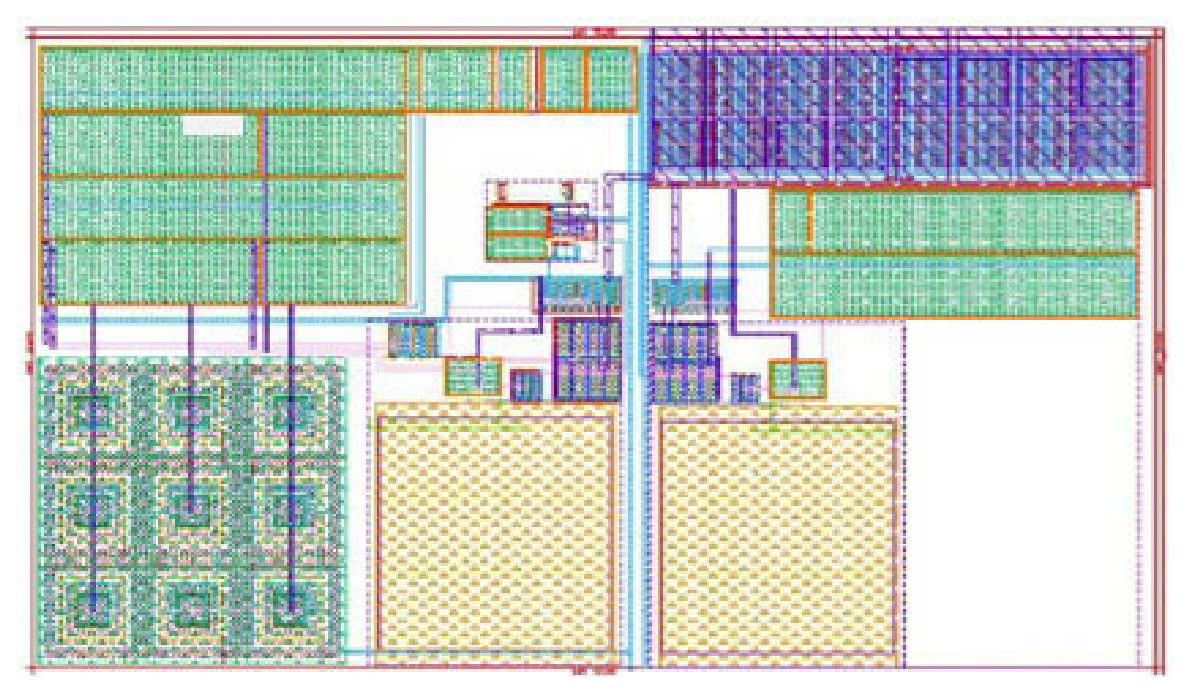
\epsfig{file=Fig/LDO_tsmc90_MR_1.eps,width=7.5cm}
    %  \caption{Original LDO layout on tsmc90nm}
    %  \label{fig:Original_LDO}
    %  \end{center}
    %\end{figure}

    \begin{figure}[ht]
      \centering
      \begin{subfigure}[t]{0.4\textwidth}
      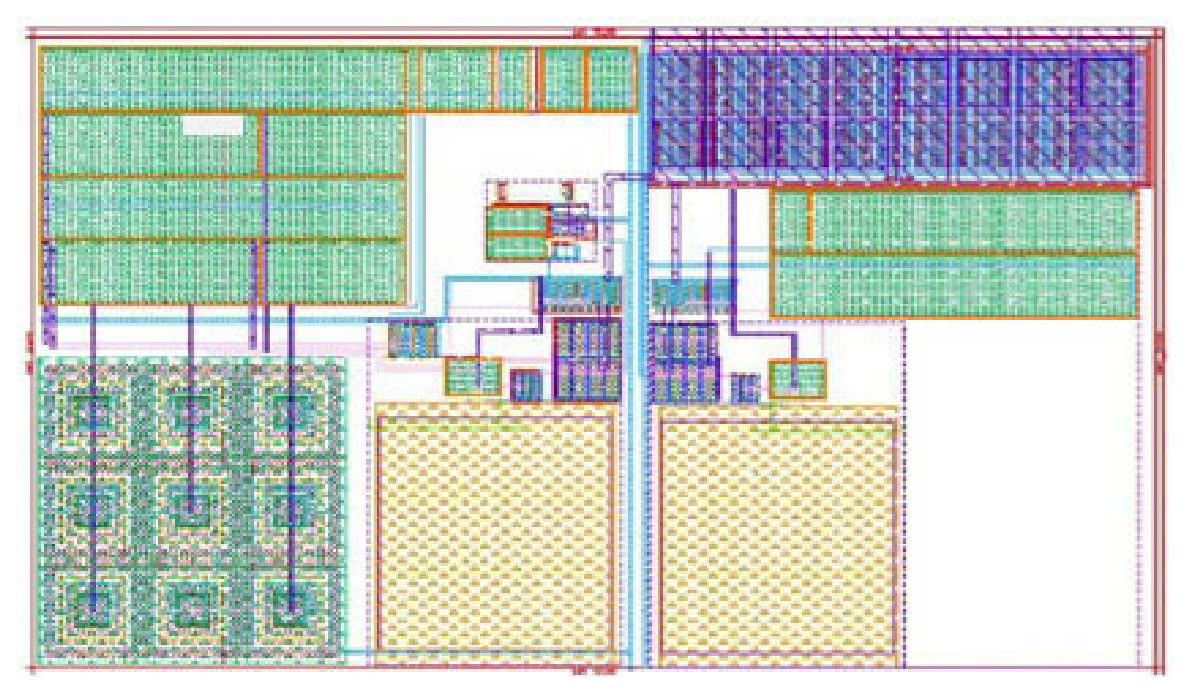
\includegraphics[width=\textwidth,angle=90]{Fig/LDO_tsmc90_MR_1.eps}
      \caption{Original LDO layout on tsmc90nm}\label{fig:Original_LDO}
      \end{subfigure}
      \begin{subfigure}[t]{0.4\textwidth}
      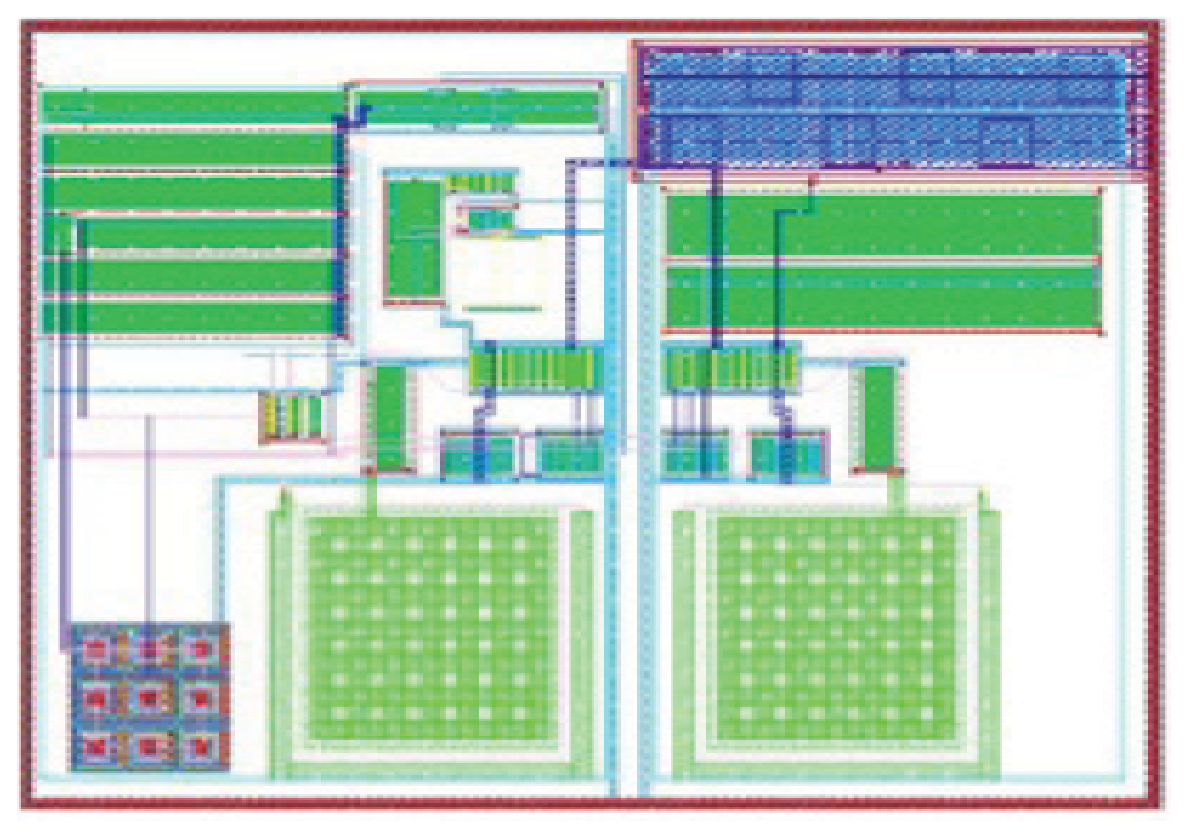
\includegraphics[width=\textwidth,angle=90]{Fig/LDO_umc90_PlFuRtCDT_1.eps}
      \caption{\cite{msc-bhattacharya-tcad06}+\cite{Chin_DMR_ICCAD2013} on umc90nm}\label{subfig:LDO_umc90_PlFuRtCDT}
      \end{subfigure}
      \begin{subfigure}[t]{0.4\textwidth}
      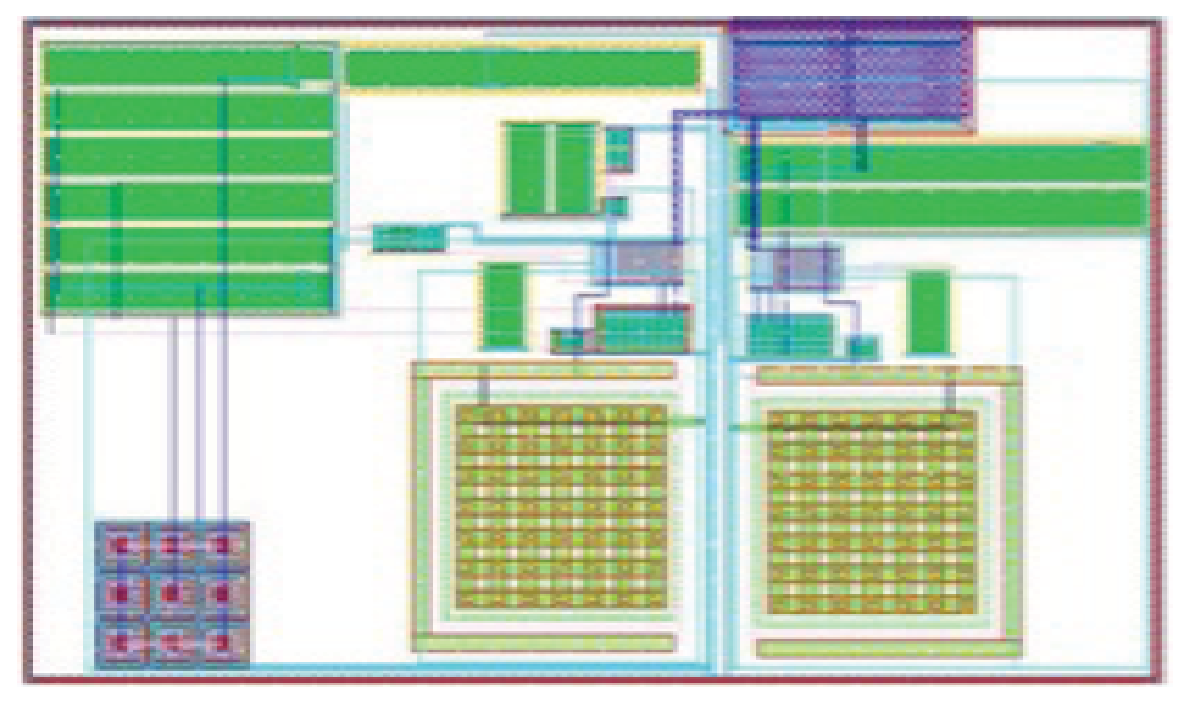
\includegraphics[width=\textwidth,angle=90]{Fig/LDO_umc65_PlFuRtCDT_1.eps}
      \caption{\cite{msc-bhattacharya-tcad06}+\cite{Chin_DMR_ICCAD2013} on umc65nm }\label{subfig:LDO_umc65_PlFuRtCDT}
      \end{subfigure}
      \begin{subfigure}[t]{0.4\textwidth}
      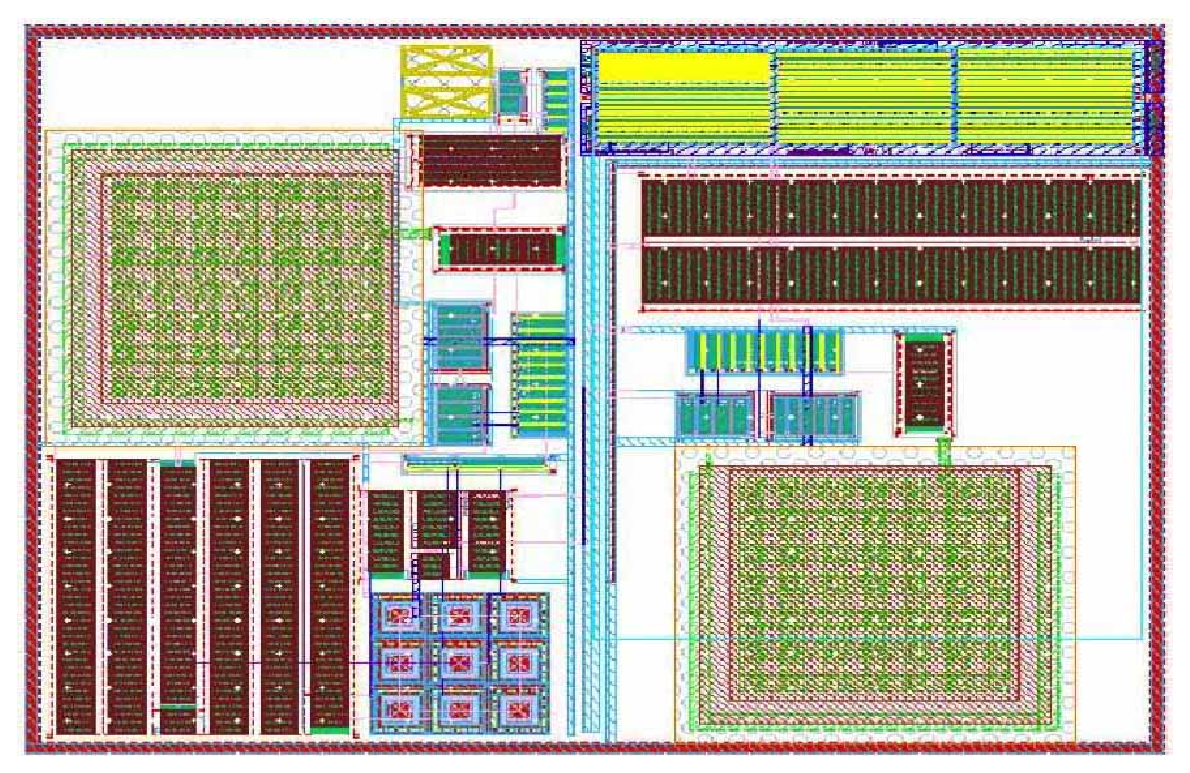
\includegraphics[width=\textwidth]{Fig/LDO_umc90_PlFxRtCDT.eps}
      \caption{Our approach on umc90nm }\label{subfig:LDO_umc90_PlFxRtCDT}
      \end{subfigure}
      \begin{subfigure}[t]{0.4\textwidth}
      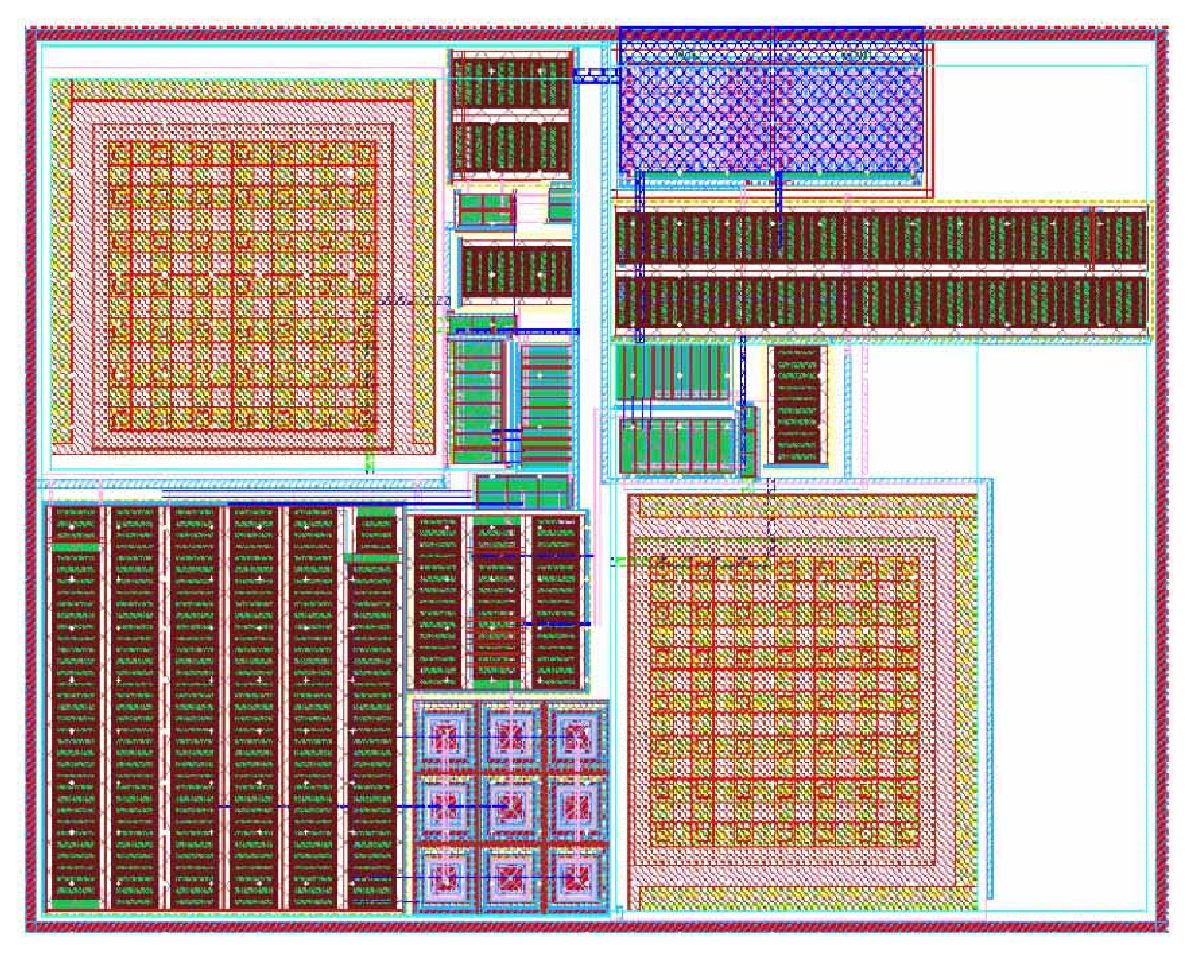
\includegraphics[width=\textwidth]{Fig/LDO_umc65_PlFxRtCDT.eps}
      \caption{Our approach on umc65nm }\label{subfig:LDO_umc65_PlFxRtCDT}  
      \end{subfigure}
    \caption{LDO from origin to migration with \cite{msc-bhattacharya-tcad06}+\cite{Chin_DMR_ICCAD2013} and our approach}\label{fig:LDO}
    \end{figure}


    

    In Table~\ref{table:HierProto}, row 3-14 show the feasibility on our approach for each technology with the simulation results, and all the testing circuit satisfy the performance specification. For umc90nm technology, our approach earns better performance on quiescent current, minimum $R_{on}$, $V_{out}$ settling time, temperature, power efficiency, $V_{drop-out}$, $\Delta V_{out-transient}$ and phase margin than \cite{msc-bhattacharya-tcad06}+\cite{Chin_DMR_ICCAD2013}. At the same time, for umc65nm technology, our approach earns better performance on dropout voltage, quiescent current, $Minimum R_{on}$, $V_{out}$ settling time, $\Delta V_{out-transient}$, open loop gain and phase margin. We can observe that even the other parts of simulation data are not notable. For the purpose to generate layout prototypes efficiently, a migrated layout with flexible placement topology dominate most of the performance metrics. Our approach framework accomplishes qualified layout results with higher productivity.

  
    For the reusability of the framework, we have collected further statistics in routing issues. As revealed in row 15-17 at Table~\ref{table:HierProto}, the overall WL, auto-gen WL and routing completeness represent the routing behavior among 5 layout results. In the original layout on tsmc90nm. The routing is accomplished manually with wirelength 2426.73$\mu m$, and the wirelength for the other two technologies with the same placement topology (\cite{msc-bhattacharya-tcad06}+\cite{Chin_DMR_ICCAD2013}) are 2122.814$\mu m$ and 1590.84$\mu m$. Meanwhile, our approach on umc90nm and umc65nm result in 1579.09$\mu m$ and 1308$\mu m$, respectively. We can observe that our approach takes more routing wirelength, but also earns more routing completeness with 78.8\% and 83.9\% on umc90nm and umc65nm. We can tell that the lost routing completeness rate is mostly made from the lost of triangles during {\it Crossing Graph Updating} in Section~\ref{sec:updateG}. The loss of triangles indicates the destruction of planar relationship. The more triangles miss, the more wires need to be reconnected. Even though our approach obtains worse routing completeness than \cite{msc-bhattacharya-tcad06}+\cite{Chin_DMR_ICCAD2013}, the performance is averagely better and the area is obviously compact than \cite{msc-bhattacharya-tcad06}+\cite{Chin_DMR_ICCAD2013}.

  In brief, the experimental results show that our approach with multiple placement topologies enlarges the solution space, CDT-based-migrated routing raises the routing reusability out of preservation and wire segment refinement explores the better performance. Meanwhile, the compelling speed-up of design time indicates the productivity for analog design.



